\documentclass[11pt,a4paper]{article}
\usepackage{booktabs,longtable,geometry,array,xcolor,microtype,graphicx,hyperref}
\geometry{margin=2cm}
\renewcommand{\arraystretch}{1.25}
\hypersetup{colorlinks=true,linkcolor=blue,urlcolor=blue}
\title{\textbf{Supplementary Material}}
\author{}
\date{}
\begin{document}
\maketitle
\tableofcontents
\clearpage
\documentclass[11pt,a4paper]{article}
\usepackage{booktabs,longtable,geometry,array,xcolor,microtype}
\geometry{margin=2cm}
\renewcommand{\arraystretch}{1.25}
\begin{document}
\section*{S1 — Full Donor Cohort}
All donors included in the study with group assignment, age, sex, and cell counts
per condition (collagen-coated vs.\ uncoated wells). Hypertension status and aortic
diameter (where available) were obtained from clinical records and are listed in the
main methods section. Donor 03Asc-54 was excluded from Part~2 statistical tests
due to missing BAV comparison data (noted in the main text).
\vspace{1em}
\begin{longtable}{llcccccc}
\toprule
Donor & Group & Age & Sex & $N_{+\text{coll}}$ & $N_{\text{no coll}}$ & $N_{\text{total}}$ \\
\midrule
\endfirsthead
\toprule Donor & Group & Age & Sex & $N_{+\text{coll}}$ & $N_{\text{no coll}}$ & $N_{\text{total}}$ \\\midrule\endhead
\bottomrule\endfoot
\multicolumn{7}{l}{\textit{Healthy}} \\
  01ASC-0180 & Healthy & 62 & Male & 10 & 10 & 20 \\
  01Asc-0231 & Healthy & 60 & Male & 5 & 5 & 10 \\
  01Asc-0232 & Healthy & 49 & Male & 5 & 5 & 10 \\
  01Asc-230 & Healthy & 63 & Female & 5 & 5 & 10 \\
  01C-0096 & Healthy & 53 & Male & 5 & 5 & 10 \\
  01C-0097 & Healthy & 57 & Female & 5 & 5 & 10 \\
  01C-0113 & Healthy & 64 & Female & 5 & 5 & 10 \\
  01C-0117 & Healthy & 46 & Female & 5 & 5 & 10 \\
  01C-202 & Healthy & 78 & Female & 5 & 5 & 10 \\
  01C-222 & Healthy & 66 & Male & 5 & 5 & 10 \\
\midrule
\multicolumn{7}{l}{\textit{TAA}} \\
  03Asc-0024 & TAA & 62 & Male & 5 & 10 & 15 \\
  03Asc-0043 & TAA & 70 & Male & 5 & 5 & 10 \\
  03Asc-0051 & TAA & 65 & Female & 5 & 5 & 10 \\
  03Asc-0054 & TAA & 75 & Female & 0 & 5 & 5 \\
  03Asc-0055 & TAA & 66 & Female & 5 & 5 & 10 \\
  03Asc-0056 & TAA & 44 & Female & 5 & 5 & 10 \\
  03Asc-0057 & TAA & 73 & Female & 5 & 5 & 10 \\
  03Rt-0045 & TAA & 75 & Male & 5 & 5 & 10 \\
\midrule
\multicolumn{7}{l}{\textit{BAV}} \\
  02Asc-0017 & BAV & 73 & Male & 6 & 5 & 11 \\
  02Asc-0021 & BAV & 61 & Male & 0 & 6 & 6 \\
  02Asc-0029 & BAV & 64 & Female & 5 & 5 & 10 \\
  02Asc-0049 & BAV & 58 & Female & 5 & 6 & 11 \\
  02Asc-0077 & BAV & -- & Male & 6 & 6 & 12 \\
\midrule
  \textbf{Total} & & & & & & 240 \\
\bottomrule
\end{longtable}
\end{document}

\clearpage
\documentclass[11pt,a4paper]{article}
\usepackage{booktabs,longtable,geometry,array,xcolor,microtype}
\geometry{margin=2cm}
\renewcommand{\arraystretch}{1.25}
\begin{document}
\section*{S2 — Shapiro--Wilk Normality Test Results}
Shapiro--Wilk test $p$-values for all 30 features in each group.
Features with $p < 0.05$ in at least one group failed normality
and received Mann--Whitney~U (cell level) or Wilcoxon signed-rank (patient level)
tests instead of Welch $t$-tests. All 30 features failed normality in at least one
group; the adaptive testing strategy therefore applied to the full feature set.
\vspace{1em}
\begin{longtable}{lrrr}
\toprule
Feature & BAV & Healthy & TAA \\
 & \multicolumn{3}{c}{Shapiro--Wilk $p$-value} \\
\midrule\endfirsthead
\toprule Feature & BAV & Healthy & TAA\\\midrule\endhead
\bottomrule\endfoot
  Actin Convex Hull Volume $\mu$m$^{3}$ & 0.277 & $<$0.001$^{*}$ & $<$0.001$^{*}$ \\
  Actin Extent ratio & 0.013$^{*}$ & $<$0.001$^{*}$ & $<$0.001$^{*}$ \\
  Actin Fractional Anisotropy ratio & 0.002$^{*}$ & $<$0.001$^{*}$ & $<$0.001$^{*}$ \\
  Actin Intermediate Axis $\mu$m & 0.003$^{*}$ & $<$0.001$^{*}$ & $<$0.001$^{*}$ \\
  Actin Major Axis $\mu$m & 0.206 & 0.842 & 0.576 \\
  Actin Minor Axis $\mu$m & 0.072 & 0.285 & 0.172 \\
  Actin Skeleton Length $\mu$m & $<$0.001$^{*}$ & $<$0.001$^{*}$ & $<$0.001$^{*}$ \\
  Actin Solidity ratio & 0.043$^{*}$ & 0.007$^{*}$ & 0.047$^{*}$ \\
  Actin Volume $\mu$m$^{3}$ & $<$0.001$^{*}$ & $<$0.001$^{*}$ & $<$0.001$^{*}$ \\
  Mito Branch Count n & $<$0.001$^{*}$ & $<$0.001$^{*}$ & $<$0.001$^{*}$ \\
  Mito Cyclomatic Number n & $<$0.001$^{*}$ & $<$0.001$^{*}$ & $<$0.001$^{*}$ \\
  Mito Fragment Count n & $<$0.001$^{*}$ & $<$0.001$^{*}$ & $<$0.001$^{*}$ \\
  Mito Junction Count n & $<$0.001$^{*}$ & $<$0.001$^{*}$ & $<$0.001$^{*}$ \\
  Mito Max Fragment Sphericity ratio & 0.008$^{*}$ & $<$0.001$^{*}$ & $<$0.001$^{*}$ \\
  Mito Mean Branch Length $\mu$m & 0.040$^{*}$ & $<$0.001$^{*}$ & $<$0.001$^{*}$ \\
  Mito Mean Fragment Sphericity ratio & 0.009$^{*}$ & 0.484 & 0.153 \\
  Mito Mean Fragment Volume $\mu$m$^{3}$ & $<$0.001$^{*}$ & $<$0.001$^{*}$ & $<$0.001$^{*}$ \\
  Mito Mean Tortuosity ratio & 0.006$^{*}$ & $<$0.001$^{*}$ & $<$0.001$^{*}$ \\
  Mito Min Fragment Sphericity ratio & 0.002$^{*}$ & $<$0.001$^{*}$ & 0.004$^{*}$ \\
  Mito Sphericity ratio & 0.100 & $<$0.001$^{*}$ & 0.442 \\
  Mito Std Fragment Sphericity ratio & 0.114 & $<$0.001$^{*}$ & 0.145 \\
  Mito Surface Area $\mu$m$^{2}$ & $<$0.001$^{*}$ & $<$0.001$^{*}$ & $<$0.001$^{*}$ \\
  Mito Total Network Length $\mu$m & $<$0.001$^{*}$ & $<$0.001$^{*}$ & $<$0.001$^{*}$ \\
  Mito Volume $\mu$m$^{3}$ & $<$0.001$^{*}$ & $<$0.001$^{*}$ & $<$0.001$^{*}$ \\
  Nucleus Circularity ratio & $<$0.001$^{*}$ & $<$0.001$^{*}$ & $<$0.001$^{*}$ \\
  Nucleus Elongation ratio & 0.085 & $<$0.001$^{*}$ & $<$0.001$^{*}$ \\
  Nucleus Flatness ratio & 0.053 & $<$0.001$^{*}$ & 0.089 \\
  Nucleus Solidity ratio & $<$0.001$^{*}$ & $<$0.001$^{*}$ & $<$0.001$^{*}$ \\
  Nucleus Sphericity ratio & 0.887 & $<$0.001$^{*}$ & $<$0.001$^{*}$ \\
  Nucleus Volume $\mu$m$^{3}$ & $<$0.001$^{*}$ & $<$0.001$^{*}$ & $<$0.001$^{*}$ \\
\bottomrule
\multicolumn{4}{l}{\footnotesize $^{*}p < 0.05$: failed normality.} \\
\end{longtable}
\end{document}

\clearpage
\documentclass[11pt,a4paper]{article}
\usepackage{booktabs,longtable,geometry,array,xcolor,microtype}
\geometry{margin=2cm}
\renewcommand{\arraystretch}{1.25}
\begin{document}
\section*{S3 — Full Cohen's~$d$ Table: Part~1: Healthy vs.\ TAA}
All 30 features for healthy vs.\ diseased (TAA), at both cell and patient level,
raw and age-residualised. $q$: BH-FDR adjusted $p$-value. $^{*}$: $q < 0.05$.
\vspace{1em}
\begin{longtable}{lrrrrrrrr}
\toprule
 & \multicolumn{2}{c}{Cell (raw)} & \multicolumn{2}{c}{Cell (age-corr.)} & \multicolumn{2}{c}{Patient (raw)} & \multicolumn{2}{c}{Patient (age-corr.)} \\
\cmidrule(lr){2-3}\cmidrule(lr){4-5}\cmidrule(lr){6-7}\cmidrule(lr){8-9}
Feature & $d$ & $q$ & $d$ & $q$ & $d$ & $q$ & $d$ & $q$ \\
\midrule\endfirsthead
\toprule Feature & $d$ & $q$ & $d$ & $q$ & $d$ & $q$ & $d$ & $q$ \\\midrule\endhead
\bottomrule\endfoot
\multicolumn{9}{l}{\textit{Actin}} \\
  Convex Hull Volume $\mu$m$^{3}$ & +0.24 & 0.260 & +0.33 & 0.145 & +0.35 & 0.549 & +0.48 & 0.638 \\
  Extent ratio & -1.00$^{*}$ & $<$0.001 & -0.87$^{*}$ & $<$0.001 & -1.25 & 0.084 & -1.10 & 0.191 \\
  Fractional Anisotropy ratio & -0.13 & 0.545 & -0.11 & 0.688 & -0.19 & 0.714 & -0.16 & 0.720 \\
  Intermediate Axis $\mu$m & +0.09 & 0.370 & +0.18 & 0.241 & +0.14 & 0.549 & +0.25 & 0.666 \\
  Major Axis $\mu$m & +0.00 & 0.980 & +0.11 & 0.688 & +0.08 & 0.608 & +0.24 & 0.666 \\
  Minor Axis $\mu$m & -0.26 & 0.265 & -0.28 & 0.239 & -0.27 & 0.635 & -0.30 & 0.666 \\
  Skeleton Length $\mu$m & +0.69$^{*}$ & $<$0.001 & +0.49$^{*}$ & 0.003 & +0.95 & 0.290 & +0.86 & 0.300 \\
  Solidity ratio & -1.15$^{*}$ & $<$0.001 & -1.04$^{*}$ & $<$0.001 & -1.62$^{*}$ & 0.038 & -1.46 & 0.095 \\
  Volume $\mu$m$^{3}$ & -0.48 & 0.085 & -0.36 & 0.241 & -0.44 & 0.524 & -0.28 & 0.666 \\
\midrule
\multicolumn{9}{l}{\textit{Mito}} \\
  Branch Count n & +0.64$^{*}$ & 0.002 & +0.53 & 0.087 & +0.68 & 0.185 & +0.55 & 0.666 \\
  Cyclomatic Number n & -0.60$^{*}$ & 0.016 & -0.48 & 0.099 & -0.64 & 0.290 & -0.50 & 0.666 \\
  Fragment Count n & +0.54$^{*}$ & 0.002 & +0.49$^{*}$ & 0.015 & +0.73 & 0.183 & +0.66 & 0.406 \\
  Junction Count n & +0.64$^{*}$ & 0.002 & +0.52 & 0.078 & +0.67 & 0.290 & +0.54 & 0.666 \\
  Max Fragment Sphericity ratio & +0.26 & 0.139 & +0.21 & 0.823 & +0.53 & 0.460 & +0.45 & 0.638 \\
  Mean Branch Length $\mu$m & -0.37 & 0.110 & -0.20 & 0.689 & -0.34 & 0.778 & -0.16 & 0.720 \\
  Mean Fragment Sphericity ratio & -0.25 & 0.286 & -0.20 & 0.374 & -0.22 & 0.687 & -0.16 & 0.720 \\
  Mean Fragment Volume $\mu$m$^{3}$ & +0.37 & 0.335 & +0.41 & 0.203 & +0.52 & 0.608 & +0.58 & 0.638 \\
  Mean Tortuosity ratio & -0.01 & 0.487 & -0.22 & 0.200 & -0.05 & 0.608 & -0.29 & 0.666 \\
  Min Fragment Sphericity ratio & -0.96$^{*}$ & $<$0.001 & -0.90$^{*}$ & $<$0.001 & -1.32 & 0.084 & -1.23 & 0.154 \\
  Sphericity ratio & -0.86$^{*}$ & $<$0.001 & -0.76$^{*}$ & $<$0.001 & -1.09 & 0.183 & -0.97 & 0.268 \\
  Std Fragment Sphericity ratio & +0.05 & 0.335 & +0.10 & 0.241 & +0.09 & 0.524 & +0.15 & 0.638 \\
  Surface Area $\mu$m$^{2}$ & +0.46$^{*}$ & 0.005 & +0.43$^{*}$ & 0.024 & +0.53 & 0.290 & +0.49 & 0.615 \\
  Total Network Length $\mu$m & +0.63$^{*}$ & $<$0.001 & +0.53 & 0.087 & +0.68 & 0.183 & +0.56 & 0.666 \\
  Volume $\mu$m$^{3}$ & +0.34 & 0.063 & +0.42$^{*}$ & 0.025 & +0.40 & 0.352 & +0.50 & 0.300 \\
\midrule
\multicolumn{9}{l}{\textit{Nucleus}} \\
  Circularity ratio & -0.19 & 0.507 & +0.33 & 0.953 & -- & -- & -- & -- \\
  Elongation ratio & -0.18 & 0.545 & -0.15 & 0.738 & -0.42 & 0.549 & -0.35 & 0.666 \\
  Flatness ratio & -0.22 & 0.335 & -0.26 & 0.243 & -0.32 & 0.608 & -0.43 & 0.666 \\
  Solidity ratio & +0.39 & 0.139 & +0.36 & 0.231 & +0.70 & 0.290 & +0.64 & 0.638 \\
  Sphericity ratio & +0.48$^{*}$ & 0.029 & +0.33 & 0.953 & +0.67 & 0.290 & +0.49 & 0.638 \\
  Volume $\mu$m$^{3}$ & -0.14 & 0.980 & +0.02 & 0.509 & -0.19 & 0.805 & +0.05 & 0.666 \\
\bottomrule
\multicolumn{9}{l}{\footnotesize $^{*}q < 0.05$ (BH-FDR).} \\
\end{longtable}
\end{document}

\clearpage
\documentclass[11pt,a4paper]{article}
\usepackage{booktabs,longtable,geometry,array,xcolor,microtype}
\geometry{margin=2cm}
\renewcommand{\arraystretch}{1.25}
\begin{document}
\section*{S4 — Full Cohen's~$d$ Table: Part~2: TAV-ATAA vs.\ BAV-ATAA}
All 30 features for TAV-ATAA vs.\ BAV-ATAA, at both cell and patient level,
raw and age-residualised. $q$: BH-FDR adjusted $p$-value. $^{*}$: $q < 0.05$.
\vspace{1em}
\begin{longtable}{lrrrrrrrr}
\toprule
 & \multicolumn{2}{c}{Cell (raw)} & \multicolumn{2}{c}{Cell (age-corr.)} & \multicolumn{2}{c}{Patient (raw)} & \multicolumn{2}{c}{Patient (age-corr.)} \\
\cmidrule(lr){2-3}\cmidrule(lr){4-5}\cmidrule(lr){6-7}\cmidrule(lr){8-9}
Feature & $d$ & $q$ & $d$ & $q$ & $d$ & $q$ & $d$ & $q$ \\
\midrule\endfirsthead
\toprule Feature & $d$ & $q$ & $d$ & $q$ & $d$ & $q$ & $d$ & $q$ \\\midrule\endhead
\bottomrule\endfoot
\multicolumn{9}{l}{\textit{Actin}} \\
  Convex Hull Volume $\mu$m$^{3}$ & +0.47$^{*}$ & 0.032 & +0.47 & 0.056 & +0.48 & 0.463 & +0.48 & 0.521 \\
  Extent ratio & +1.28$^{*}$ & $<$0.001 & +1.28$^{*}$ & $<$0.001 & +1.99$^{*}$ & 0.011 & +2.05$^{*}$ & 0.007 \\
  Fractional Anisotropy ratio & -0.18 & 0.314 & -0.19 & 0.307 & -0.21 & 0.705 & -0.22 & 0.705 \\
  Intermediate Axis $\mu$m & +0.69$^{*}$ & 0.018 & +0.68$^{*}$ & 0.020 & +0.79 & 0.234 & +0.78 & 0.275 \\
  Major Axis $\mu$m & +0.92$^{*}$ & $<$0.001 & +0.90$^{*}$ & 0.004 & +1.17 & 0.073 & +1.16 & 0.124 \\
  Minor Axis $\mu$m & -0.30 & 0.281 & -0.32 & 0.251 & -0.39 & 0.643 & -0.42 & 0.521 \\
  Skeleton Length $\mu$m & -2.53$^{*}$ & $<$0.001 & -3.11$^{*}$ & $<$0.001 & -2.99$^{*}$ & 0.013 & -4.56$^{*}$ & 0.004 \\
  Solidity ratio & +0.83$^{*}$ & 0.002 & +0.83$^{*}$ & 0.002 & +1.39$^{*}$ & 0.040 & +1.41 & 0.079 \\
  Volume $\mu$m$^{3}$ & +1.03$^{*}$ & $<$0.001 & +1.04$^{*}$ & $<$0.001 & +1.05 & 0.094 & +1.10 & 0.153 \\
\midrule
\multicolumn{9}{l}{\textit{Mito}} \\
  Branch Count n & -0.97$^{*}$ & $<$0.001 & -0.97$^{*}$ & $<$0.001 & -1.03$^{*}$ & 0.009 & -1.05$^{*}$ & 0.025 \\
  Cyclomatic Number n & +1.14$^{*}$ & $<$0.001 & +1.15$^{*}$ & $<$0.001 & +1.25$^{*}$ & 0.016 & +1.29$^{*}$ & 0.025 \\
  Fragment Count n & +0.04 & 0.314 & +0.05 & 0.573 & +0.02 & 0.767 & +0.03 & 0.705 \\
  Junction Count n & -1.03$^{*}$ & $<$0.001 & -1.03$^{*}$ & $<$0.001 & -1.10$^{*}$ & 0.009 & -1.12$^{*}$ & 0.025 \\
  Max Fragment Sphericity ratio & -1.45$^{*}$ & $<$0.001 & -1.45$^{*}$ & $<$0.001 & -1.87$^{*}$ & 0.016 & -1.87$^{*}$ & 0.011 \\
  Mean Branch Length $\mu$m & +3.66$^{*}$ & $<$0.001 & +4.31$^{*}$ & $<$0.001 & +3.97$^{*}$ & 0.009 & +5.31$^{*}$ & 0.004 \\
  Mean Fragment Sphericity ratio & -0.35 & 0.434 & -0.37 & 0.414 & -0.45 & 1.000 & -0.46 & 1.000 \\
  Mean Fragment Volume $\mu$m$^{3}$ & +0.27 & 0.718 & +0.26 & 0.707 & +0.29 & 0.981 & +0.29 & 0.922 \\
  Mean Tortuosity ratio & -3.19$^{*}$ & $<$0.001 & -3.55$^{*}$ & $<$0.001 & -3.36$^{*}$ & 0.013 & -3.96$^{*}$ & 0.004 \\
  Min Fragment Sphericity ratio & +0.69$^{*}$ & 0.006 & +0.68$^{*}$ & 0.004 & +1.11 & 0.117 & +1.08 & 0.100 \\
  Sphericity ratio & +0.56 & 0.098 & +0.55 & 0.056 & +0.83 & 0.408 & +0.86 & 0.234 \\
  Std Fragment Sphericity ratio & -0.92$^{*}$ & $<$0.001 & -0.94$^{*}$ & $<$0.001 & -1.56$^{*}$ & 0.021 & -1.61$^{*}$ & 0.046 \\
  Surface Area $\mu$m$^{2}$ & +0.06 & 0.932 & +0.06 & 0.975 & -0.01 & 0.981 & -0.01 & 1.000 \\
  Total Network Length $\mu$m & -0.83$^{*}$ & $<$0.001 & -0.83$^{*}$ & $<$0.001 & -0.90$^{*}$ & 0.016 & -0.90 & 0.079 \\
  Volume $\mu$m$^{3}$ & +0.41 & 0.434 & +0.41 & 0.414 & +0.39 & 0.643 & +0.39 & 0.767 \\
\midrule
\multicolumn{9}{l}{\textit{Nucleus}} \\
  Circularity ratio & +0.23 & 0.434 & -0.11 & 0.689 & -- & -- & -- & -- \\
  Elongation ratio & +0.84$^{*}$ & $<$0.001 & +0.85$^{*}$ & $<$0.001 & +1.71$^{*}$ & 0.021 & +1.75$^{*}$ & 0.025 \\
  Flatness ratio & +0.28 & 0.381 & +0.30 & 0.442 & +0.44 & 0.609 & +0.47 & 0.581 \\
  Solidity ratio & +0.06 & 0.884 & +0.05 & 0.573 & +0.17 & 1.000 & +0.16 & 0.981 \\
  Sphericity ratio & -3.45$^{*}$ & $<$0.001 & -3.59$^{*}$ & $<$0.001 & -4.20$^{*}$ & 0.011 & -4.60$^{*}$ & 0.011 \\
  Volume $\mu$m$^{3}$ & +0.95$^{*}$ & $<$0.001 & +0.96$^{*}$ & $<$0.001 & +1.31$^{*}$ & 0.030 & +1.41$^{*}$ & 0.035 \\
\bottomrule
\multicolumn{9}{l}{\footnotesize $^{*}q < 0.05$ (BH-FDR).} \\
\end{longtable}
\end{document}

\clearpage
\documentclass[11pt,a4paper]{article}
\usepackage{booktabs,longtable,geometry,array,xcolor,microtype}
\geometry{margin=2cm}
\renewcommand{\arraystretch}{1.25}
\begin{document}
\section*{S5 — Full LMM Output: Part~1 (Healthy vs.\ TAA)}
Complete linear mixed model results for all 30 features.
Model: \textit{Feature} $\sim$ Disease $+$ Collagen $+$ Disease:Collagen $+$ Age $+$ (1\,|\,Donor).
$q$: BH-FDR across features within each term. $^{*}$: $q < 0.05$.
\vspace{1em}
\begin{longtable}{llrrrr}
\toprule
Feature & Term & Coef. & $p$ & $q$ & Sig. \\
\midrule\endfirsthead
\toprule Feature & Term & Coef. & $p$ & $q$ & Sig. \\\midrule\endhead
\bottomrule\endfoot
\multicolumn{6}{l}{\textit{Actin}} \\
  Convex Hull Volume $\mu$m$^{3}$ & Disease & +10787.554 & 0.335 & 0.547 &  \\
   & Collagen & -1755.115 & 0.669 & 0.946 &  \\
   & Interaction & -2280.072 & 0.698 & 0.890 &  \\
   & Age & -393.891 & 0.447 & 0.648 &  \\
  Extent ratio & Disease & -0.036 & 0.005 & 0.074 &  \\
   & Collagen & -0.010 & 0.205 & 0.684 &  \\
   & Interaction & +0.027 & 0.015 & 0.219 &  \\
   & Age & -0.001 & 0.058 & 0.420 &  \\
  Fractional Anisotropy ratio & Disease & -0.008 & 0.567 & 0.658 &  \\
   & Collagen & -0.001 & 0.897 & 0.946 &  \\
   & Interaction & +0.007 & 0.641 & 0.890 &  \\
   & Age & +0.000 & 0.895 & 0.932 &  \\
  Intermediate Axis $\mu$m & Disease & +4.055 & 0.552 & 0.658 &  \\
   & Collagen & -0.190 & 0.946 & 0.946 &  \\
   & Interaction & -0.202 & 0.960 & 0.978 &  \\
   & Age & -0.292 & 0.351 & 0.535 &  \\
  Major Axis $\mu$m & Disease & +4.125 & 0.698 & 0.778 &  \\
   & Collagen & +2.154 & 0.662 & 0.946 &  \\
   & Interaction & +3.489 & 0.620 & 0.890 &  \\
   & Age & -0.481 & 0.318 & 0.535 &  \\
  Minor Axis $\mu$m & Disease & -0.043 & 0.507 & 0.658 &  \\
   & Collagen & -0.035 & 0.208 & 0.684 &  \\
   & Interaction & +0.008 & 0.833 & 0.895 &  \\
   & Age & +0.001 & 0.693 & 0.886 &  \\
  Skeleton Length $\mu$m & Disease & +8187.930 & 0.077 & 0.328 &  \\
   & Collagen & -2842.725 & 0.307 & 0.742 &  \\
   & Interaction & +5461.859 & 0.169 & 0.446 &  \\
   & Age & +1180.987 & $<$0.001 & $<$0.001 & $^{*}$ \\
  Solidity ratio & Disease & -0.095 & $<$0.001 & 0.010 & $^{*}$ \\
   & Collagen & -0.020 & 0.246 & 0.684 &  \\
   & Interaction & +0.054 & 0.031 & 0.262 &  \\
   & Age & -0.002 & 0.112 & 0.430 &  \\
  Volume $\mu$m$^{3}$ & Disease & -2103.305 & 0.339 & 0.547 &  \\
   & Collagen & -2183.266 & 0.016 & 0.231 &  \\
   & Interaction & +2715.726 & 0.036 & 0.262 &  \\
   & Age & -139.333 & 0.167 & 0.430 &  \\
\midrule
\multicolumn{6}{l}{\textit{Mito}} \\
  Branch Count n & Disease & +10000.774 & 0.138 & 0.400 &  \\
   & Collagen & +941.364 & 0.656 & 0.946 &  \\
   & Interaction & -5403.194 & 0.074 & 0.358 &  \\
   & Age & +437.717 & 0.164 & 0.430 &  \\
  Cyclomatic Number n & Disease & -2145.887 & 0.204 & 0.455 &  \\
   & Collagen & -101.782 & 0.848 & 0.946 &  \\
   & Interaction & +1253.011 & 0.100 & 0.390 &  \\
   & Age & -106.084 & 0.178 & 0.430 &  \\
  Fragment Count n & Disease & +139.920 & 0.267 & 0.523 &  \\
   & Collagen & +79.509 & 0.259 & 0.684 &  \\
   & Interaction & +153.456 & 0.128 & 0.411 &  \\
   & Age & +8.422 & 0.131 & 0.430 &  \\
  Junction Count n & Disease & +11470.709 & 0.152 & 0.400 &  \\
   & Collagen & +832.345 & 0.729 & 0.946 &  \\
   & Interaction & -6349.069 & 0.065 & 0.358 &  \\
   & Age & +504.090 & 0.178 & 0.430 &  \\
  Max Fragment Sphericity ratio & Disease & +0.018 & 0.436 & 0.658 &  \\
   & Collagen & -0.016 & 0.135 & 0.684 &  \\
   & Interaction & +0.014 & 0.344 & 0.713 &  \\
   & Age & +0.001 & 0.235 & 0.455 &  \\
  Mean Branch Length $\mu$m & Disease & -0.167 & 0.726 & 0.780 &  \\
   & Collagen & +0.156 & 0.001 & 0.038 & $^{*}$ \\
   & Interaction & -0.018 & 0.796 & 0.895 &  \\
   & Age & -0.034 & 0.133 & 0.430 &  \\
  Mean Fragment Sphericity ratio & Disease & -0.014 & 0.546 & 0.658 &  \\
   & Collagen & -0.009 & 0.439 & 0.849 &  \\
   & Interaction & -0.004 & 0.833 & 0.895 &  \\
   & Age & +0.000 & 0.932 & 0.932 &  \\
  Mean Fragment Volume $\mu$m$^{3}$ & Disease & +21.264 & 0.079 & 0.328 &  \\
   & Collagen & +6.829 & 0.354 & 0.790 &  \\
   & Interaction & -29.990 & 0.004 & 0.126 &  \\
   & Age & -0.657 & 0.213 & 0.441 &  \\
  Mean Tortuosity ratio & Disease & -0.019 & 0.536 & 0.658 &  \\
   & Collagen & -0.014 & 0.068 & 0.661 &  \\
   & Interaction & -0.005 & 0.656 & 0.890 &  \\
   & Age & +0.002 & 0.106 & 0.430 &  \\
  Min Fragment Sphericity ratio & Disease & -0.033 & 0.016 & 0.158 &  \\
   & Collagen & -0.002 & 0.769 & 0.946 &  \\
   & Interaction & +0.010 & 0.303 & 0.676 &  \\
   & Age & -0.000 & 0.703 & 0.886 &  \\
  Sphericity ratio & Disease & -0.019 & 0.069 & 0.328 &  \\
   & Collagen & +0.001 & 0.877 & 0.946 &  \\
   & Interaction & -0.003 & 0.597 & 0.890 &  \\
   & Age & -0.000 & 0.323 & 0.535 &  \\
  Std Fragment Sphericity ratio & Disease & +0.002 & 0.777 & 0.805 &  \\
   & Collagen & -0.004 & 0.143 & 0.684 &  \\
   & Interaction & +0.002 & 0.706 & 0.890 &  \\
   & Age & -0.000 & 0.801 & 0.930 &  \\
  Surface Area $\mu$m$^{2}$ & Disease & +10394.734 & 0.144 & 0.400 &  \\
   & Collagen & -431.077 & 0.876 & 0.946 &  \\
   & Interaction & -2527.382 & 0.524 & 0.890 &  \\
   & Age & +103.029 & 0.753 & 0.910 &  \\
  Total Network Length $\mu$m & Disease & +10151.315 & 0.124 & 0.400 &  \\
   & Collagen & +654.531 & 0.761 & 0.946 &  \\
   & Interaction & -4948.481 & 0.108 & 0.390 &  \\
   & Age & +390.344 & 0.204 & 0.441 &  \\
  Volume $\mu$m$^{3}$ & Disease & +2406.222 & 0.183 & 0.442 &  \\
   & Collagen & -304.192 & 0.654 & 0.946 &  \\
   & Interaction & -417.287 & 0.668 & 0.890 &  \\
   & Age & -79.122 & 0.343 & 0.535 &  \\
\midrule
\multicolumn{6}{l}{\textit{Nucleus}} \\
  Elongation ratio & Disease & -2.426 & 0.535 & 0.658 &  \\
   & Collagen & +2.902 & 0.254 & 0.684 &  \\
   & Interaction & +0.100 & 0.978 & 0.978 &  \\
   & Age & -0.026 & 0.877 & 0.932 &  \\
  Flatness ratio & Disease & -0.023 & 0.334 & 0.547 &  \\
   & Collagen & -0.020 & 0.401 & 0.831 &  \\
   & Interaction & +0.046 & 0.162 & 0.446 &  \\
   & Age & +0.001 & 0.479 & 0.661 &  \\
  Solidity ratio & Disease & +0.054 & 0.060 & 0.328 &  \\
   & Collagen & +0.007 & 0.746 & 0.946 &  \\
   & Interaction & -0.011 & 0.701 & 0.890 &  \\
   & Age & -0.000 & 0.932 & 0.932 &  \\
  Sphericity ratio & Disease & +0.111 & 0.271 & 0.523 &  \\
   & Collagen & -0.003 & 0.936 & 0.946 &  \\
   & Interaction & -0.017 & 0.773 & 0.895 &  \\
   & Age & +0.009 & 0.053 & 0.420 &  \\
  Volume $\mu$m$^{3}$ & Disease & +19.142 & 0.950 & 0.950 &  \\
   & Collagen & -217.022 & 0.141 & 0.684 &  \\
   & Interaction & +223.303 & 0.285 & 0.676 &  \\
   & Age & -31.379 & 0.022 & 0.318 &  \\
\bottomrule
\multicolumn{6}{l}{\footnotesize $^{*}q < 0.05$ (BH-FDR).} \\
\end{longtable}
\end{document}

\clearpage
\documentclass[11pt,a4paper]{article}
\usepackage{booktabs,longtable,geometry,array,xcolor,microtype}
\geometry{margin=2cm}
\renewcommand{\arraystretch}{1.25}
\begin{document}
\section*{S5 — Full LMM Output: Part~2 (TAV-ATAA vs.\ BAV-ATAA)}
Complete linear mixed model results for all 30 features.
Model: \textit{Feature} $\sim$ Disease $+$ Collagen $+$ Disease:Collagen $+$ Age $+$ (1\,|\,Donor).
$q$: BH-FDR across features within each term. $^{*}$: $q < 0.05$.
\vspace{1em}
\begin{longtable}{llrrrr}
\toprule
Feature & Term & Coef. & $p$ & $q$ & Sig. \\
\midrule\endfirsthead
\toprule Feature & Term & Coef. & $p$ & $q$ & Sig. \\\midrule\endhead
\bottomrule\endfoot
\multicolumn{6}{l}{\textit{Actin}} \\
  Convex Hull Volume $\mu$m$^{3}$ & Disease & +20366.072 & 0.177 & 0.234 &  \\
   & Collagen & -4071.875 & 0.333 & 0.572 &  \\
   & Interaction & +18253.005 & 0.035 & 0.150 &  \\
   & Age & -488.198 & 0.436 & 0.641 &  \\
  Extent ratio & Disease & +0.054 & $<$0.001 & $<$0.001 & $^{*}$ \\
   & Collagen & +0.018 & 0.010 & 0.109 &  \\
   & Interaction & -0.045 & 0.002 & 0.053 &  \\
   & Age & -0.000 & 0.432 & 0.641 &  \\
  Fractional Anisotropy ratio & Disease & -0.017 & 0.281 & 0.352 &  \\
   & Collagen & +0.004 & 0.658 & 0.789 &  \\
   & Interaction & +0.007 & 0.732 & 0.813 &  \\
   & Age & -0.000 & 0.942 & 0.942 &  \\
  Intermediate Axis $\mu$m & Disease & +20.646 & 0.017 & 0.057 &  \\
   & Collagen & -0.172 & 0.960 & 0.963 &  \\
   & Interaction & -0.805 & 0.909 & 0.935 &  \\
   & Age & -0.161 & 0.645 & 0.758 &  \\
  Major Axis $\mu$m & Disease & +27.427 & 0.028 & 0.071 &  \\
   & Collagen & +5.677 & 0.218 & 0.503 &  \\
   & Interaction & +6.603 & 0.486 & 0.648 &  \\
   & Age & -0.419 & 0.410 & 0.641 &  \\
  Minor Axis $\mu$m & Disease & -0.030 & 0.690 & 0.770 &  \\
   & Collagen & -0.028 & 0.299 & 0.572 &  \\
   & Interaction & +0.120 & 0.028 & 0.150 &  \\
   & Age & -0.002 & 0.436 & 0.641 &  \\
  Skeleton Length $\mu$m & Disease & -29380.283 & $<$0.001 & $<$0.001 & $^{*}$ \\
   & Collagen & +2515.284 & 0.322 & 0.572 &  \\
   & Interaction & -4319.534 & 0.407 & 0.648 &  \\
   & Age & +1067.522 & $<$0.001 & $<$0.001 & $^{*}$ \\
  Solidity ratio & Disease & +0.051 & 0.025 & 0.067 &  \\
   & Collagen & +0.035 & 0.013 & 0.109 &  \\
   & Interaction & -0.081 & 0.004 & 0.053 &  \\
   & Age & -0.000 & 0.674 & 0.758 &  \\
  Volume $\mu$m$^{3}$ & Disease & +6989.496 & 0.006 & 0.024 & $^{*}$ \\
   & Collagen & +587.332 & 0.553 & 0.709 &  \\
   & Interaction & -722.881 & 0.722 & 0.813 &  \\
   & Age & -89.106 & 0.390 & 0.641 &  \\
\midrule
\multicolumn{6}{l}{\textit{Mito}} \\
  Branch Count n & Disease & -17671.726 & 0.079 & 0.136 &  \\
   & Collagen & -4487.361 & 0.040 & 0.149 &  \\
   & Interaction & +4285.469 & 0.341 & 0.648 &  \\
   & Age & +496.676 & 0.240 & 0.638 &  \\
  Cyclomatic Number n & Disease & +4802.231 & 0.045 & 0.097 &  \\
   & Collagen & +1153.517 & 0.031 & 0.133 &  \\
   & Interaction & -1190.690 & 0.281 & 0.617 &  \\
   & Age & -128.385 & 0.201 & 0.638 &  \\
  Fragment Count n & Disease & +30.769 & 0.871 & 0.901 &  \\
   & Collagen & +232.844 & 0.007 & 0.109 &  \\
   & Interaction & -379.984 & 0.031 & 0.150 &  \\
   & Age & +7.812 & 0.295 & 0.638 &  \\
  Junction Count n & Disease & -21550.867 & 0.068 & 0.136 &  \\
   & Collagen & -5534.301 & 0.027 & 0.133 &  \\
   & Interaction & +5502.813 & 0.288 & 0.617 &  \\
   & Age & +581.644 & 0.242 & 0.638 &  \\
  Max Fragment Sphericity ratio & Disease & -0.069 & $<$0.001 & 0.003 & $^{*}$ \\
   & Collagen & -0.000 & 0.963 & 0.963 &  \\
   & Interaction & -0.026 & 0.187 & 0.560 &  \\
   & Age & +0.001 & 0.250 & 0.638 &  \\
  Mean Branch Length $\mu$m & Disease & +2.731 & $<$0.001 & $<$0.001 & $^{*}$ \\
   & Collagen & +0.138 & 0.049 & 0.164 &  \\
   & Interaction & -0.109 & 0.451 & 0.648 &  \\
   & Age & -0.044 & 0.008 & 0.115 &  \\
  Mean Fragment Sphericity ratio & Disease & +0.001 & 0.944 & 0.944 &  \\
   & Collagen & -0.011 & 0.345 & 0.572 &  \\
   & Interaction & +0.012 & 0.602 & 0.752 &  \\
   & Age & -0.000 & 0.682 & 0.758 &  \\
  Mean Fragment Volume $\mu$m$^{3}$ & Disease & +34.033 & 0.138 & 0.197 &  \\
   & Collagen & -23.348 & 0.022 & 0.131 &  \\
   & Interaction & -19.113 & 0.360 & 0.648 &  \\
   & Age & -0.945 & 0.298 & 0.638 &  \\
  Mean Tortuosity ratio & Disease & -0.161 & $<$0.001 & $<$0.001 & $^{*}$ \\
   & Collagen & -0.019 & 0.014 & 0.109 &  \\
   & Interaction & +0.038 & 0.016 & 0.122 &  \\
   & Age & +0.002 & 0.054 & 0.538 &  \\
  Min Fragment Sphericity ratio & Disease & +0.023 & 0.082 & 0.136 &  \\
   & Collagen & +0.008 & 0.111 & 0.288 &  \\
   & Interaction & -0.001 & 0.935 & 0.935 &  \\
   & Age & -0.000 & 0.646 & 0.758 &  \\
  Sphericity ratio & Disease & +0.011 & 0.180 & 0.234 &  \\
   & Collagen & -0.003 & 0.362 & 0.572 &  \\
   & Interaction & +0.017 & 0.005 & 0.053 &  \\
   & Age & -0.000 & 0.156 & 0.638 &  \\
  Std Fragment Sphericity ratio & Disease & -0.013 & 0.045 & 0.097 &  \\
   & Collagen & -0.002 & 0.459 & 0.656 &  \\
   & Interaction & -0.008 & 0.207 & 0.563 &  \\
   & Age & +0.000 & 0.566 & 0.739 &  \\
  Surface Area $\mu$m$^{2}$ & Disease & +4725.196 & 0.668 & 0.770 &  \\
   & Collagen & -2916.494 & 0.439 & 0.656 &  \\
   & Interaction & -5273.816 & 0.496 & 0.648 &  \\
   & Age & +133.654 & 0.767 & 0.793 &  \\
  Total Network Length $\mu$m & Disease & -14934.354 & 0.132 & 0.197 &  \\
   & Collagen & -4319.861 & 0.056 & 0.168 &  \\
   & Interaction & +3291.789 & 0.480 & 0.648 &  \\
   & Age & +459.248 & 0.270 & 0.638 &  \\
  Volume $\mu$m$^{3}$ & Disease & +5483.329 & 0.076 & 0.136 &  \\
   & Collagen & -696.089 & 0.567 & 0.709 &  \\
   & Interaction & -2841.704 & 0.256 & 0.617 &  \\
   & Age & -95.061 & 0.445 & 0.641 &  \\
\midrule
\multicolumn{6}{l}{\textit{Nucleus}} \\
  Circularity ratio & Disease & -0.033 & 0.792 & 0.849 &  \\
   & Collagen & +0.022 & 0.729 & 0.810 &  \\
   & Interaction & -0.051 & 0.497 & 0.648 &  \\
   & Age & +0.003 & 0.513 & 0.699 &  \\
  Elongation ratio & Disease & +7.928 & 0.021 & 0.062 &  \\
   & Collagen & +2.981 & 0.115 & 0.288 &  \\
   & Interaction & -7.728 & 0.043 & 0.163 &  \\
   & Age & +0.048 & 0.710 & 0.761 &  \\
  Flatness ratio & Disease & +0.049 & 0.122 & 0.192 &  \\
   & Collagen & +0.027 & 0.263 & 0.563 &  \\
   & Interaction & -0.067 & 0.173 & 0.560 &  \\
   & Age & +0.002 & 0.123 & 0.638 &  \\
  Solidity ratio & Disease & +0.011 & 0.693 & 0.770 &  \\
   & Collagen & -0.005 & 0.722 & 0.810 &  \\
   & Interaction & -0.013 & 0.630 & 0.756 &  \\
   & Age & -0.001 & 0.449 & 0.641 &  \\
  Sphericity ratio & Disease & -0.594 & $<$0.001 & $<$0.001 & $^{*}$ \\
   & Collagen & -0.021 & 0.503 & 0.686 &  \\
   & Interaction & +0.051 & 0.417 & 0.648 &  \\
   & Age & +0.007 & 0.095 & 0.638 &  \\
  Volume $\mu$m$^{3}$ & Disease & +1580.750 & $<$0.001 & 0.001 & $^{*}$ \\
   & Collagen & +21.650 & 0.928 & 0.963 &  \\
   & Interaction & +41.985 & 0.931 & 0.935 &  \\
   & Age & -21.200 & 0.201 & 0.638 &  \\
\bottomrule
\multicolumn{6}{l}{\footnotesize $^{*}q < 0.05$ (BH-FDR).} \\
\end{longtable}
\end{document}

\clearpage
\documentclass[11pt,a4paper]{article}
\usepackage{booktabs,longtable,geometry,array,xcolor,microtype}
\geometry{margin=2cm}
\renewcommand{\arraystretch}{1.25}
\begin{document}
\section*{S6 — Intraclass Correlation Coefficients (ICC)}
ICC values quantify the proportion of total variance explained by donor identity 
(random intercept) in the linear mixed model. These values were computed from the 
fitted variance components: $\text{ICC} = \sigma^2_{\text{donor}} / (\sigma^2_{\text{donor}} + \sigma^2_{\text{residual}})$.

\textbf{Note:} ICC extraction requires re-running the LMM with variance component 
output enabled on the analysis server. This table will be populated upon re-run.
\end{document}

\clearpage
\documentclass[11pt,a4paper]{article}
\usepackage{booktabs,longtable,geometry,array,xcolor,microtype}
\geometry{margin=2cm}
\renewcommand{\arraystretch}{1.25}
\begin{document}
\section*{S7 — Full Collagen Rescue Results: Part~1 (Healthy vs.\ TAA)}
Effect of collagen coating within each disease group at cell level (Mann--Whitney~U)
and patient level (Wilcoxon signed-rank). $d$: Cohen's~$d$. $q$: BH-FDR. $^{*}$: $q<0.05$.
\vspace{1em}
\subsection*{Cell level}
\begin{longtable}{llrrr}
\toprule
Feature & Group & $d$ & $q$ & Sig. \\
\midrule\endfirsthead
\toprule Feature & Group & $d$ & $q$ & Sig. \\\midrule\endhead
\bottomrule\endfoot
\multicolumn{5}{l}{\textit{Actin}} \\
  Convex Hull Volume $\mu$m$^{3}$ & Healthy & -0.06 & 0.925 &  \\
  Extent ratio & Healthy & -0.18 & 0.925 &  \\
  Fractional Anisotropy ratio & Healthy & -0.02 & 0.925 &  \\
  Intermediate Axis $\mu$m & Healthy & -0.01 & 0.945 &  \\
  Major Axis $\mu$m & Healthy & +0.06 & 0.925 &  \\
  Minor Axis $\mu$m & Healthy & -0.18 & 0.925 &  \\
  Skeleton Length $\mu$m & Healthy & -0.15 & 0.925 &  \\
  Solidity ratio & Healthy & -0.16 & 0.925 &  \\
  Volume $\mu$m$^{3}$ & Healthy & -0.29 & 0.925 &  \\
\midrule
\multicolumn{5}{l}{\textit{Mito}} \\
  Branch Count n & Healthy & +0.09 & 0.925 &  \\
  Cyclomatic Number n & Healthy & -0.03 & 0.925 &  \\
  Fragment Count n & Healthy & +0.27 & 0.925 &  \\
  Junction Count n & Healthy & +0.07 & 0.925 &  \\
  Max Fragment Sphericity ratio & Healthy & -0.20 & 0.925 &  \\
  Mean Branch Length $\mu$m & Healthy & +0.11 & 0.925 &  \\
  Mean Fragment Sphericity ratio & Healthy & -0.12 & 0.925 &  \\
  Mean Fragment Volume $\mu$m$^{3}$ & Healthy & +0.22 & 0.970 &  \\
  Mean Tortuosity ratio & Healthy & -0.15 & 0.925 &  \\
  Min Fragment Sphericity ratio & Healthy & -0.04 & 0.925 &  \\
  Sphericity ratio & Healthy & +0.02 & 0.925 &  \\
  Std Fragment Sphericity ratio & Healthy & -0.18 & 0.925 &  \\
  Surface Area $\mu$m$^{2}$ & Healthy & -0.03 & 0.925 &  \\
  Total Network Length $\mu$m & Healthy & +0.07 & 0.925 &  \\
  Volume $\mu$m$^{3}$ & Healthy & -0.07 & 0.925 &  \\
\midrule
\multicolumn{5}{l}{\textit{Nucleus}} \\
  Circularity ratio & Healthy & +0.01 & 0.970 &  \\
  Elongation ratio & Healthy & +0.18 & 0.925 &  \\
  Flatness ratio & Healthy & -0.18 & 0.925 &  \\
  Solidity ratio & Healthy & +0.06 & 0.945 &  \\
  Sphericity ratio & Healthy & -0.01 & 0.925 &  \\
  Volume $\mu$m$^{3}$ & Healthy & -0.18 & 0.925 &  \\
\midrule
\multicolumn{5}{l}{\textit{Actin}} \\
  Convex Hull Volume $\mu$m$^{3}$ & TAA & +0.01 & 0.993 &  \\
  Extent ratio & TAA & +0.55 & 0.172 &  \\
  Fractional Anisotropy ratio & TAA & +0.04 & 0.878 &  \\
  Intermediate Axis $\mu$m & TAA & +0.12 & 0.683 &  \\
  Major Axis $\mu$m & TAA & +0.23 & 0.543 &  \\
  Minor Axis $\mu$m & TAA & -0.06 & 0.878 &  \\
  Skeleton Length $\mu$m & TAA & +0.08 & 0.873 &  \\
  Solidity ratio & TAA & +0.46 & 0.172 &  \\
  Volume $\mu$m$^{3}$ & TAA & +0.23 & 0.543 &  \\
\midrule
\multicolumn{5}{l}{\textit{Mito}} \\
  Branch Count n & TAA & -0.18 & 0.513 &  \\
  Cyclomatic Number n & TAA & +0.22 & 0.495 &  \\
  Fragment Count n & TAA & +0.45 & 0.172 &  \\
  Junction Count n & TAA & -0.20 & 0.495 &  \\
  Max Fragment Sphericity ratio & TAA & +0.04 & 0.873 &  \\
  Mean Branch Length $\mu$m & TAA & +0.26 & 0.495 &  \\
  Mean Fragment Sphericity ratio & TAA & -0.12 & 0.873 &  \\
  Mean Fragment Volume $\mu$m$^{3}$ & TAA & -0.40 & 0.325 &  \\
  Mean Tortuosity ratio & TAA & -0.36 & 0.357 &  \\
  Min Fragment Sphericity ratio & TAA & +0.21 & 0.759 &  \\
  Sphericity ratio & TAA & -0.17 & 0.761 &  \\
  Std Fragment Sphericity ratio & TAA & -0.13 & 1.000 &  \\
  Surface Area $\mu$m$^{2}$ & TAA & -0.04 & 0.993 &  \\
  Total Network Length $\mu$m & TAA & -0.16 & 0.647 &  \\
  Volume $\mu$m$^{3}$ & TAA & -0.02 & 0.873 &  \\
\midrule
\multicolumn{5}{l}{\textit{Nucleus}} \\
  Circularity ratio & TAA & +0.24 & 0.873 &  \\
  Elongation ratio & TAA & +0.21 & 0.803 &  \\
  Flatness ratio & TAA & +0.20 & 0.543 &  \\
  Solidity ratio & TAA & -0.02 & 0.993 &  \\
  Sphericity ratio & TAA & -0.15 & 0.873 &  \\
  Volume $\mu$m$^{3}$ & TAA & +0.11 & 0.845 &  \\
\bottomrule
\end{longtable}
\subsection*{Patient level}
\begin{longtable}{llrrr}
\toprule
Feature & Group & $d$ & $q$ & Sig. \\
\midrule\endfirsthead
\toprule Feature & Group & $d$ & $q$ & Sig. \\\midrule\endhead
\bottomrule\endfoot
\multicolumn{5}{l}{\textit{Actin}} \\
  Convex Hull Volume $\mu$m$^{3}$ & Healthy & +0.02 & 1.000 &  \\
  Extent ratio & Healthy & -0.20 & 1.000 &  \\
  Fractional Anisotropy ratio & Healthy & +0.01 & 1.000 &  \\
  Intermediate Axis $\mu$m & Healthy & -0.01 & 1.000 &  \\
  Major Axis $\mu$m & Healthy & +0.10 & 1.000 &  \\
  Minor Axis $\mu$m & Healthy & -0.15 & 1.000 &  \\
  Skeleton Length $\mu$m & Healthy & -0.08 & 1.000 &  \\
  Solidity ratio & Healthy & -0.18 & 1.000 &  \\
  Volume $\mu$m$^{3}$ & Healthy & -0.26 & 0.967 &  \\
\midrule
\multicolumn{5}{l}{\textit{Mito}} \\
  Branch Count n & Healthy & +0.19 & 1.000 &  \\
  Cyclomatic Number n & Healthy & -0.08 & 1.000 &  \\
  Fragment Count n & Healthy & +0.35 & 1.000 &  \\
  Junction Count n & Healthy & +0.13 & 1.000 &  \\
  Max Fragment Sphericity ratio & Healthy & -0.26 & 1.000 &  \\
  Mean Branch Length $\mu$m & Healthy & +0.09 & 1.000 &  \\
  Mean Fragment Sphericity ratio & Healthy & -0.13 & 1.000 &  \\
  Mean Fragment Volume $\mu$m$^{3}$ & Healthy & +0.37 & 1.000 &  \\
  Mean Tortuosity ratio & Healthy & -0.14 & 1.000 &  \\
  Min Fragment Sphericity ratio & Healthy & -0.05 & 1.000 &  \\
  Sphericity ratio & Healthy & +0.04 & 1.000 &  \\
  Std Fragment Sphericity ratio & Healthy & -0.24 & 1.000 &  \\
  Surface Area $\mu$m$^{2}$ & Healthy & -0.01 & 1.000 &  \\
  Total Network Length $\mu$m & Healthy & +0.16 & 1.000 &  \\
  Volume $\mu$m$^{3}$ & Healthy & -0.05 & 1.000 &  \\
\midrule
\multicolumn{5}{l}{\textit{Nucleus}} \\
  Circularity ratio & Healthy & +0.00 & 1.000 &  \\
  Elongation ratio & Healthy & +0.24 & 1.000 &  \\
  Flatness ratio & Healthy & -0.41 & 1.000 &  \\
  Solidity ratio & Healthy & +0.07 & 1.000 &  \\
  Sphericity ratio & Healthy & +0.00 & 1.000 &  \\
  Volume $\mu$m$^{3}$ & Healthy & -0.23 & 0.967 &  \\
\midrule
\multicolumn{5}{l}{\textit{Actin}} \\
  Convex Hull Volume $\mu$m$^{3}$ & TAA & -0.16 & 0.804 &  \\
  Extent ratio & TAA & +0.96 & 0.387 &  \\
  Fractional Anisotropy ratio & TAA & +0.26 & 1.000 &  \\
  Intermediate Axis $\mu$m & TAA & -0.08 & 1.000 &  \\
  Major Axis $\mu$m & TAA & +0.23 & 0.804 &  \\
  Minor Axis $\mu$m & TAA & -0.25 & 0.869 &  \\
  Skeleton Length $\mu$m & TAA & +0.11 & 1.000 &  \\
  Solidity ratio & TAA & +0.74 & 0.387 &  \\
  Volume $\mu$m$^{3}$ & TAA & +0.09 & 0.893 &  \\
\midrule
\multicolumn{5}{l}{\textit{Mito}} \\
  Branch Count n & TAA & -0.20 & 0.697 &  \\
  Cyclomatic Number n & TAA & +0.21 & 0.387 &  \\
  Fragment Count n & TAA & +0.49 & 0.710 &  \\
  Junction Count n & TAA & -0.21 & 0.387 &  \\
  Max Fragment Sphericity ratio & TAA & -0.13 & 0.948 &  \\
  Mean Branch Length $\mu$m & TAA & +0.15 & 0.561 &  \\
  Mean Fragment Sphericity ratio & TAA & -0.42 & 1.000 &  \\
  Mean Fragment Volume $\mu$m$^{3}$ & TAA & -0.64 & 0.387 &  \\
  Mean Tortuosity ratio & TAA & -0.27 & 0.697 &  \\
  Min Fragment Sphericity ratio & TAA & +0.30 & 0.561 &  \\
  Sphericity ratio & TAA & -0.18 & 0.962 &  \\
  Std Fragment Sphericity ratio & TAA & -0.23 & 0.869 &  \\
  Surface Area $\mu$m$^{2}$ & TAA & -0.14 & 0.863 &  \\
  Total Network Length $\mu$m & TAA & -0.20 & 0.697 &  \\
  Volume $\mu$m$^{3}$ & TAA & -0.15 & 0.893 &  \\
\midrule
\multicolumn{5}{l}{\textit{Nucleus}} \\
  Circularity ratio & TAA & +0.00 & 1.000 &  \\
  Elongation ratio & TAA & +0.61 & 0.804 &  \\
  Flatness ratio & TAA & +0.22 & 0.893 &  \\
  Solidity ratio & TAA & -0.14 & 0.962 &  \\
  Sphericity ratio & TAA & -0.10 & 0.893 &  \\
  Volume $\mu$m$^{3}$ & TAA & -0.02 & 1.000 &  \\
\bottomrule
\end{longtable}
\end{document}

\clearpage
\documentclass[11pt,a4paper]{article}
\usepackage{booktabs,longtable,geometry,array,xcolor,microtype}
\geometry{margin=2cm}
\renewcommand{\arraystretch}{1.25}
\begin{document}
\section*{S7 — Full Collagen Rescue Results: Part~2 (TAV-ATAA vs.\ BAV-ATAA)}
Effect of collagen coating within each disease group at cell level (Mann--Whitney~U)
and patient level (Wilcoxon signed-rank). $d$: Cohen's~$d$. $q$: BH-FDR. $^{*}$: $q<0.05$.
\vspace{1em}
\subsection*{Cell level}
\begin{longtable}{llrrr}
\toprule
Feature & Group & $d$ & $q$ & Sig. \\
\midrule\endfirsthead
\toprule Feature & Group & $d$ & $q$ & Sig. \\\midrule\endhead
\bottomrule\endfoot
\multicolumn{5}{l}{\textit{Actin}} \\
  Convex Hull Volume $\mu$m$^{3}$ & TAA & +0.01 & 0.993 &  \\
  Extent ratio & TAA & +0.55 & 0.172 &  \\
  Fractional Anisotropy ratio & TAA & +0.04 & 0.878 &  \\
  Intermediate Axis $\mu$m & TAA & +0.12 & 0.683 &  \\
  Major Axis $\mu$m & TAA & +0.23 & 0.543 &  \\
  Minor Axis $\mu$m & TAA & -0.06 & 0.878 &  \\
  Skeleton Length $\mu$m & TAA & +0.08 & 0.873 &  \\
  Solidity ratio & TAA & +0.46 & 0.172 &  \\
  Volume $\mu$m$^{3}$ & TAA & +0.23 & 0.543 &  \\
\midrule
\multicolumn{5}{l}{\textit{Mito}} \\
  Branch Count n & TAA & -0.18 & 0.513 &  \\
  Cyclomatic Number n & TAA & +0.22 & 0.495 &  \\
  Fragment Count n & TAA & +0.45 & 0.172 &  \\
  Junction Count n & TAA & -0.20 & 0.495 &  \\
  Max Fragment Sphericity ratio & TAA & +0.04 & 0.873 &  \\
  Mean Branch Length $\mu$m & TAA & +0.26 & 0.495 &  \\
  Mean Fragment Sphericity ratio & TAA & -0.12 & 0.873 &  \\
  Mean Fragment Volume $\mu$m$^{3}$ & TAA & -0.40 & 0.325 &  \\
  Mean Tortuosity ratio & TAA & -0.36 & 0.357 &  \\
  Min Fragment Sphericity ratio & TAA & +0.21 & 0.759 &  \\
  Sphericity ratio & TAA & -0.17 & 0.761 &  \\
  Std Fragment Sphericity ratio & TAA & -0.13 & 1.000 &  \\
  Surface Area $\mu$m$^{2}$ & TAA & -0.04 & 0.993 &  \\
  Total Network Length $\mu$m & TAA & -0.16 & 0.647 &  \\
  Volume $\mu$m$^{3}$ & TAA & -0.02 & 0.873 &  \\
\midrule
\multicolumn{5}{l}{\textit{Nucleus}} \\
  Circularity ratio & TAA & +0.24 & 0.873 &  \\
  Elongation ratio & TAA & +0.21 & 0.803 &  \\
  Flatness ratio & TAA & +0.20 & 0.543 &  \\
  Solidity ratio & TAA & -0.02 & 0.993 &  \\
  Sphericity ratio & TAA & -0.15 & 0.873 &  \\
  Volume $\mu$m$^{3}$ & TAA & +0.11 & 0.845 &  \\
\midrule
\multicolumn{5}{l}{\textit{Actin}} \\
  Convex Hull Volume $\mu$m$^{3}$ & BAV & +0.30 & 0.769 &  \\
  Extent ratio & BAV & -0.46 & 0.721 &  \\
  Fractional Anisotropy ratio & BAV & +0.10 & 0.914 &  \\
  Intermediate Axis $\mu$m & BAV & +0.13 & 0.769 &  \\
  Major Axis $\mu$m & BAV & +0.44 & 0.721 &  \\
  Minor Axis $\mu$m & BAV & +0.12 & 0.914 &  \\
  Skeleton Length $\mu$m & BAV & -0.06 & 0.769 &  \\
  Solidity ratio & BAV & -0.49 & 0.721 &  \\
  Volume $\mu$m$^{3}$ & BAV & -0.11 & 0.788 &  \\
\midrule
\multicolumn{5}{l}{\textit{Mito}} \\
  Branch Count n & BAV & -0.14 & 0.769 &  \\
  Cyclomatic Number n & BAV & -0.09 & 0.897 &  \\
  Fragment Count n & BAV & -0.34 & 0.914 &  \\
  Junction Count n & BAV & -0.12 & 0.769 &  \\
  Max Fragment Sphericity ratio & BAV & -0.23 & 0.769 &  \\
  Mean Branch Length $\mu$m & BAV & -0.20 & 0.769 &  \\
  Mean Fragment Sphericity ratio & BAV & -0.01 & 0.914 &  \\
  Mean Fragment Volume $\mu$m$^{3}$ & BAV & -0.51 & 0.914 &  \\
  Mean Tortuosity ratio & BAV & +0.63 & 0.721 &  \\
  Min Fragment Sphericity ratio & BAV & +0.04 & 0.897 &  \\
  Sphericity ratio & BAV & +0.28 & 0.769 &  \\
  Std Fragment Sphericity ratio & BAV & -0.30 & 0.769 &  \\
  Surface Area $\mu$m$^{2}$ & BAV & -0.26 & 0.769 &  \\
  Total Network Length $\mu$m & BAV & -0.18 & 0.769 &  \\
  Volume $\mu$m$^{3}$ & BAV & -0.29 & 0.769 &  \\
\midrule
\multicolumn{5}{l}{\textit{Nucleus}} \\
  Circularity ratio & BAV & -0.15 & 0.769 &  \\
  Elongation ratio & BAV & -0.43 & 0.721 &  \\
  Flatness ratio & BAV & -0.12 & 0.961 &  \\
  Solidity ratio & BAV & -0.22 & 0.721 &  \\
  Sphericity ratio & BAV & +0.34 & 0.721 &  \\
  Volume $\mu$m$^{3}$ & BAV & -0.03 & 0.769 &  \\
\bottomrule
\end{longtable}
\subsection*{Patient level}
\begin{longtable}{llrrr}
\toprule
Feature & Group & $d$ & $q$ & Sig. \\
\midrule\endfirsthead
\toprule Feature & Group & $d$ & $q$ & Sig. \\\midrule\endhead
\bottomrule\endfoot
\multicolumn{5}{l}{\textit{Actin}} \\
  Convex Hull Volume $\mu$m$^{3}$ & TAA & -0.16 & 0.804 &  \\
  Extent ratio & TAA & +0.96 & 0.387 &  \\
  Fractional Anisotropy ratio & TAA & +0.26 & 1.000 &  \\
  Intermediate Axis $\mu$m & TAA & -0.08 & 1.000 &  \\
  Major Axis $\mu$m & TAA & +0.23 & 0.804 &  \\
  Minor Axis $\mu$m & TAA & -0.25 & 0.869 &  \\
  Skeleton Length $\mu$m & TAA & +0.11 & 1.000 &  \\
  Solidity ratio & TAA & +0.74 & 0.387 &  \\
  Volume $\mu$m$^{3}$ & TAA & +0.09 & 0.893 &  \\
\midrule
\multicolumn{5}{l}{\textit{Mito}} \\
  Branch Count n & TAA & -0.20 & 0.697 &  \\
  Cyclomatic Number n & TAA & +0.21 & 0.387 &  \\
  Fragment Count n & TAA & +0.49 & 0.710 &  \\
  Junction Count n & TAA & -0.21 & 0.387 &  \\
  Max Fragment Sphericity ratio & TAA & -0.13 & 0.948 &  \\
  Mean Branch Length $\mu$m & TAA & +0.15 & 0.561 &  \\
  Mean Fragment Sphericity ratio & TAA & -0.42 & 1.000 &  \\
  Mean Fragment Volume $\mu$m$^{3}$ & TAA & -0.64 & 0.387 &  \\
  Mean Tortuosity ratio & TAA & -0.27 & 0.697 &  \\
  Min Fragment Sphericity ratio & TAA & +0.30 & 0.561 &  \\
  Sphericity ratio & TAA & -0.18 & 0.962 &  \\
  Std Fragment Sphericity ratio & TAA & -0.23 & 0.869 &  \\
  Surface Area $\mu$m$^{2}$ & TAA & -0.14 & 0.863 &  \\
  Total Network Length $\mu$m & TAA & -0.20 & 0.697 &  \\
  Volume $\mu$m$^{3}$ & TAA & -0.15 & 0.893 &  \\
\midrule
\multicolumn{5}{l}{\textit{Nucleus}} \\
  Circularity ratio & TAA & +0.00 & 1.000 &  \\
  Elongation ratio & TAA & +0.61 & 0.804 &  \\
  Flatness ratio & TAA & +0.22 & 0.893 &  \\
  Solidity ratio & TAA & -0.14 & 0.962 &  \\
  Sphericity ratio & TAA & -0.10 & 0.893 &  \\
  Volume $\mu$m$^{3}$ & TAA & -0.02 & 1.000 &  \\
\midrule
\multicolumn{5}{l}{\textit{Actin}} \\
  Convex Hull Volume $\mu$m$^{3}$ & BAV & +0.35 & 1.000 &  \\
  Extent ratio & BAV & -0.70 & 1.000 &  \\
  Fractional Anisotropy ratio & BAV & +0.21 & 1.000 &  \\
  Intermediate Axis $\mu$m & BAV & +0.07 & 1.000 &  \\
  Major Axis $\mu$m & BAV & +0.54 & 1.000 &  \\
  Minor Axis $\mu$m & BAV & +0.22 & 1.000 &  \\
  Skeleton Length $\mu$m & BAV & -0.14 & 1.000 &  \\
  Solidity ratio & BAV & -0.87 & 1.000 &  \\
  Volume $\mu$m$^{3}$ & BAV & -0.06 & 1.000 &  \\
\midrule
\multicolumn{5}{l}{\textit{Mito}} \\
  Branch Count n & BAV & -0.24 & 1.000 &  \\
  Cyclomatic Number n & BAV & -0.18 & 1.000 &  \\
  Fragment Count n & BAV & -0.74 & 1.000 &  \\
  Junction Count n & BAV & -0.19 & 1.000 &  \\
  Max Fragment Sphericity ratio & BAV & -0.14 & 1.000 &  \\
  Mean Branch Length $\mu$m & BAV & +0.04 & 1.000 &  \\
  Mean Fragment Sphericity ratio & BAV & +0.11 & 1.000 &  \\
  Mean Fragment Volume $\mu$m$^{3}$ & BAV & -0.51 & 1.000 &  \\
  Mean Tortuosity ratio & BAV & +0.99 & 1.000 &  \\
  Min Fragment Sphericity ratio & BAV & +0.21 & 1.000 &  \\
  Sphericity ratio & BAV & +0.59 & 1.000 &  \\
  Std Fragment Sphericity ratio & BAV & -0.52 & 1.000 &  \\
  Surface Area $\mu$m$^{2}$ & BAV & -0.31 & 1.000 &  \\
  Total Network Length $\mu$m & BAV & -0.24 & 1.000 &  \\
  Volume $\mu$m$^{3}$ & BAV & -0.31 & 1.000 &  \\
\midrule
\multicolumn{5}{l}{\textit{Nucleus}} \\
  Circularity ratio & BAV & -0.31 & 1.000 &  \\
  Elongation ratio & BAV & -1.15 & 1.000 &  \\
  Flatness ratio & BAV & +0.08 & 1.000 &  \\
  Solidity ratio & BAV & -0.46 & 1.000 &  \\
  Sphericity ratio & BAV & +0.64 & 1.000 &  \\
  Volume $\mu$m$^{3}$ & BAV & -0.04 & 1.000 &  \\
\bottomrule
\end{longtable}
\end{document}

\clearpage
\documentclass[11pt,a4paper]{article}
\usepackage{booktabs,longtable,geometry,array,xcolor,microtype}
\geometry{margin=2cm}
\renewcommand{\arraystretch}{1.25}
\begin{document}
\section*{S8 — Full Aortic Diameter Correlation Table}
Spearman's $\rho$ between each feature and aortic diameter across all 13 TAA
specimens with available diameter measurements. $q$: BH-FDR. $^{*}$: $q<0.05$.
\vspace{1em}
\subsection*{Cell level}
\begin{longtable}{lrrrr}
\toprule
Feature & $\rho$ & $p$ & $n$ & $q$ \\
\midrule\endfirsthead
\toprule Feature & $\rho$ & $p$ & $n$ & $q$ \\\midrule\endhead
\bottomrule\endfoot
\multicolumn{5}{l}{\textit{Actin}} \\
  Convex Hull Volume $\mu$m$^{3}$ & -0.780$^{*}$ & $<$0.001 & 71 & $<$0.001 \\
  Extent ratio & -0.474$^{*}$ & $<$0.001 & 71 & $<$0.001 \\
  Fractional Anisotropy ratio & +0.437$^{*}$ & $<$0.001 & 71 & $<$0.001 \\
  Intermediate Axis $\mu$m & -0.637$^{*}$ & $<$0.001 & 71 & $<$0.001 \\
  Major Axis $\mu$m & -0.478$^{*}$ & $<$0.001 & 71 & $<$0.001 \\
  Minor Axis $\mu$m & -0.399$^{*}$ & $<$0.001 & 71 & 0.001 \\
  Skeleton Length $\mu$m & +0.304$^{*}$ & 0.010 & 71 & 0.018 \\
  Solidity ratio & -0.037 & 0.762 & 71 & 0.816 \\
  Volume $\mu$m$^{3}$ & -0.757$^{*}$ & $<$0.001 & 71 & $<$0.001 \\
\midrule
\multicolumn{5}{l}{\textit{Mito}} \\
  Branch Count n & +0.270$^{*}$ & 0.023 & 71 & 0.036 \\
  Cyclomatic Number n & -0.420$^{*}$ & $<$0.001 & 71 & $<$0.001 \\
  Fragment Count n & -0.292$^{*}$ & 0.014 & 71 & 0.023 \\
  Junction Count n & +0.356$^{*}$ & 0.002 & 71 & 0.004 \\
  Max Fragment Sphericity ratio & +0.259$^{*}$ & 0.029 & 71 & 0.044 \\
  Mean Branch Length $\mu$m & -0.518$^{*}$ & $<$0.001 & 71 & $<$0.001 \\
  Mean Fragment Sphericity ratio & -0.106 & 0.378 & 71 & 0.473 \\
  Mean Fragment Volume $\mu$m$^{3}$ & -0.381$^{*}$ & 0.001 & 71 & 0.002 \\
  Mean Tortuosity ratio & +0.727$^{*}$ & $<$0.001 & 71 & $<$0.001 \\
  Min Fragment Sphericity ratio & +0.083 & 0.490 & 71 & 0.574 \\
  Sphericity ratio & +0.190 & 0.112 & 71 & 0.152 \\
  Std Fragment Sphericity ratio & +0.082 & 0.497 & 71 & 0.574 \\
  Surface Area $\mu$m$^{2}$ & -0.521$^{*}$ & $<$0.001 & 71 & $<$0.001 \\
  Total Network Length $\mu$m & +0.015 & 0.899 & 71 & 0.930 \\
  Volume $\mu$m$^{3}$ & -0.613$^{*}$ & $<$0.001 & 71 & $<$0.001 \\
\midrule
\multicolumn{5}{l}{\textit{Nucleus}} \\
  Circularity ratio & -0.019 & 0.933 & 21 & 0.933 \\
  Elongation ratio & +0.162 & 0.177 & 71 & 0.231 \\
  Flatness ratio & -0.202 & 0.091 & 71 & 0.131 \\
  Solidity ratio & -0.042 & 0.731 & 71 & 0.812 \\
  Sphericity ratio & +0.425$^{*}$ & $<$0.001 & 71 & $<$0.001 \\
  Volume $\mu$m$^{3}$ & -0.571$^{*}$ & $<$0.001 & 71 & $<$0.001 \\
\bottomrule
\end{longtable}
\subsection*{Patient level}
\begin{longtable}{lrrrr}
\toprule
Feature & $\rho$ & $p$ & $n$ & $q$ \\
\midrule\endfirsthead
\toprule Feature & $\rho$ & $p$ & $n$ & $q$ \\\midrule\endhead
\bottomrule\endfoot
\multicolumn{5}{l}{\textit{Actin}} \\
  Convex Hull Volume $\mu$m$^{3}$ & -0.928$^{*}$ & $<$0.001 & 13 & $<$0.001 \\
  Extent ratio & -0.463 & 0.111 & 13 & 0.230 \\
  Fractional Anisotropy ratio & +0.601 & 0.030 & 13 & 0.087 \\
  Intermediate Axis $\mu$m & -0.813$^{*}$ & $<$0.001 & 13 & 0.004 \\
  Major Axis $\mu$m & -0.532 & 0.061 & 13 & 0.152 \\
  Minor Axis $\mu$m & -0.691$^{*}$ & 0.009 & 13 & 0.032 \\
  Skeleton Length $\mu$m & +0.223 & 0.464 & 13 & 0.611 \\
  Solidity ratio & +0.135 & 0.660 & 13 & 0.736 \\
  Volume $\mu$m$^{3}$ & -0.904$^{*}$ & $<$0.001 & 13 & $<$0.001 \\
\midrule
\multicolumn{5}{l}{\textit{Mito}} \\
  Branch Count n & +0.306 & 0.310 & 13 & 0.473 \\
  Cyclomatic Number n & -0.529 & 0.063 & 13 & 0.152 \\
  Fragment Count n & -0.601 & 0.030 & 13 & 0.087 \\
  Junction Count n & +0.369 & 0.214 & 13 & 0.372 \\
  Max Fragment Sphericity ratio & +0.211 & 0.490 & 13 & 0.618 \\
  Mean Branch Length $\mu$m & -0.366 & 0.218 & 13 & 0.372 \\
  Mean Fragment Sphericity ratio & -0.058 & 0.851 & 13 & 0.914 \\
  Mean Fragment Volume $\mu$m$^{3}$ & -0.501 & 0.081 & 13 & 0.180 \\
  Mean Tortuosity ratio & +0.837$^{*}$ & $<$0.001 & 13 & 0.003 \\
  Min Fragment Sphericity ratio & +0.017 & 0.957 & 13 & 0.957 \\
  Sphericity ratio & +0.135 & 0.660 & 13 & 0.736 \\
  Std Fragment Sphericity ratio & +0.187 & 0.540 & 13 & 0.652 \\
  Surface Area $\mu$m$^{2}$ & -0.702$^{*}$ & 0.007 & 13 & 0.031 \\
  Total Network Length $\mu$m & +0.017 & 0.957 & 13 & 0.957 \\
  Volume $\mu$m$^{3}$ & -0.818$^{*}$ & $<$0.001 & 13 & 0.004 \\
\midrule
\multicolumn{5}{l}{\textit{Nucleus}} \\
  Elongation ratio & +0.424 & 0.149 & 13 & 0.287 \\
  Flatness ratio & -0.333 & 0.266 & 13 & 0.428 \\
  Solidity ratio & -0.292 & 0.333 & 13 & 0.483 \\
  Sphericity ratio & +0.277 & 0.360 & 13 & 0.498 \\
  Volume $\mu$m$^{3}$ & -0.716$^{*}$ & 0.006 & 13 & 0.028 \\
\bottomrule
\end{longtable}
\end{document}

\clearpage
\documentclass[11pt,a4paper]{article}
\usepackage{booktabs,longtable,geometry,array,xcolor,microtype}
\geometry{margin=2cm}
\renewcommand{\arraystretch}{1.25}
\begin{document}
\section*{S9 — Full Hypertension Analysis Results}
Cohen's~$d$ for hypertensive vs.\ normotensive donors in the TAA cohort,
at cell and patient level. $q$: BH-FDR. $^{*}$: $q<0.05$.
\vspace{1em}
\subsection*{Cell level}
\begin{longtable}{lrrrrrr}
\toprule
Feature & $n_\text{HT}$ & $n_\text{norm}$ & $d$ & $p$ & $q$ & Sig. \\
\midrule\endfirsthead
\toprule Feature & $n_\text{HT}$ & $n_\text{norm}$ & $d$ & $p$ & $q$ & Sig. \\\midrule\endhead
\bottomrule\endfoot
\multicolumn{7}{l}{\textit{Actin}} \\
  Convex Hull Volume $\mu$m$^{3}$ & 61 & 15 & -0.81 & 0.008 & 0.021 & $^{*}$ \\
  Extent ratio & 61 & 15 & -0.39 & 0.039 & 0.078 &  \\
  Fractional Anisotropy ratio & 61 & 15 & +0.31 & 0.267 & 0.341 &  \\
  Intermediate Axis $\mu$m & 61 & 15 & -0.47 & 0.103 & 0.181 &  \\
  Major Axis $\mu$m & 61 & 15 & -0.29 & 0.434 & 0.520 &  \\
  Minor Axis $\mu$m & 61 & 15 & -0.73 & 0.011 & 0.026 & $^{*}$ \\
  Skeleton Length $\mu$m & 61 & 15 & +1.02 & 0.001 & 0.005 & $^{*}$ \\
  Solidity ratio & 61 & 15 & -0.21 & 0.514 & 0.593 &  \\
  Volume $\mu$m$^{3}$ & 61 & 15 & -0.77 & 0.001 & 0.005 & $^{*}$ \\
\midrule
\multicolumn{7}{l}{\textit{Mito}} \\
  Branch Count n & 61 & 15 & +0.91 & $<$0.001 & $<$0.001 & $^{*}$ \\
  Cyclomatic Number n & 61 & 15 & -1.07 & $<$0.001 & $<$0.001 & $^{*}$ \\
  Fragment Count n & 61 & 15 & +0.48 & 0.092 & 0.173 &  \\
  Junction Count n & 61 & 15 & +0.97 & $<$0.001 & $<$0.001 & $^{*}$ \\
  Max Fragment Sphericity ratio & 61 & 15 & +0.34 & 0.221 & 0.316 &  \\
  Mean Branch Length $\mu$m & 61 & 15 & -1.30 & $<$0.001 & $<$0.001 & $^{*}$ \\
  Mean Fragment Sphericity ratio & 61 & 15 & -0.60 & 0.036 & 0.076 &  \\
  Mean Fragment Volume $\mu$m$^{3}$ & 61 & 15 & +0.09 & 0.686 & 0.735 &  \\
  Mean Tortuosity ratio & 61 & 15 & +1.72 & $<$0.001 & $<$0.001 & $^{*}$ \\
  Min Fragment Sphericity ratio & 61 & 15 & -0.66 & 0.009 & 0.024 & $^{*}$ \\
  Sphericity ratio & 61 & 15 & -0.95 & 0.002 & 0.008 & $^{*}$ \\
  Std Fragment Sphericity ratio & 61 & 15 & +0.20 & 0.794 & 0.821 &  \\
  Surface Area $\mu$m$^{2}$ & 61 & 15 & +0.35 & 0.273 & 0.341 &  \\
  Total Network Length $\mu$m & 61 & 15 & +0.85 & $<$0.001 & $<$0.001 & $^{*}$ \\
  Volume $\mu$m$^{3}$ & 61 & 15 & +0.09 & 0.896 & 0.896 &  \\
\midrule
\multicolumn{7}{l}{\textit{Nucleus}} \\
  Circularity ratio & 11 & 10 & +0.22 & 0.130 & 0.217 &  \\
  Elongation ratio & 61 & 15 & +0.15 & 0.548 & 0.609 &  \\
  Flatness ratio & 61 & 15 & +0.40 & 0.262 & 0.341 &  \\
  Solidity ratio & 61 & 15 & +0.19 & 0.187 & 0.281 &  \\
  Sphericity ratio & 61 & 15 & +0.92 & 0.007 & 0.021 & $^{*}$ \\
  Volume $\mu$m$^{3}$ & 61 & 15 & -0.17 & 0.179 & 0.281 &  \\
\bottomrule
\end{longtable}
\subsection*{Patient level}
\begin{longtable}{lrrrrrr}
\toprule
Feature & $n_\text{HT}$ & $n_\text{norm}$ & $d$ & $p$ & $q$ & Sig. \\
\midrule\endfirsthead
\toprule Feature & $n_\text{HT}$ & $n_\text{norm}$ & $d$ & $p$ & $q$ & Sig. \\\midrule\endhead
\bottomrule\endfoot
\multicolumn{7}{l}{\textit{Actin}} \\
  Convex Hull Volume $\mu$m$^{3}$ & 11 & 3 & -0.82 & 0.225 & 0.503 &  \\
  Extent ratio & 11 & 3 & -0.46 & 0.291 & 0.528 &  \\
  Fractional Anisotropy ratio & 11 & 3 & +0.46 & 0.456 & 0.671 &  \\
  Intermediate Axis $\mu$m & 11 & 3 & -0.51 & 0.456 & 0.671 &  \\
  Major Axis $\mu$m & 11 & 3 & -0.29 & 0.769 & 0.826 &  \\
  Minor Axis $\mu$m & 11 & 3 & -1.18 & 0.126 & 0.458 &  \\
  Skeleton Length $\mu$m & 11 & 3 & +1.05 & 0.291 & 0.528 &  \\
  Solidity ratio & 11 & 3 & -0.27 & 0.769 & 0.826 &  \\
  Volume $\mu$m$^{3}$ & 11 & 3 & -0.83 & 0.225 & 0.503 &  \\
\midrule
\multicolumn{7}{l}{\textit{Mito}} \\
  Branch Count n & 11 & 3 & +0.98 & 0.038 & 0.292 &  \\
  Cyclomatic Number n & 11 & 3 & -1.20 & 0.088 & 0.364 &  \\
  Fragment Count n & 11 & 3 & +0.80 & 0.225 & 0.503 &  \\
  Junction Count n & 11 & 3 & +1.05 & 0.038 & 0.292 &  \\
  Max Fragment Sphericity ratio & 11 & 3 & +0.43 & 0.532 & 0.671 &  \\
  Mean Branch Length $\mu$m & 11 & 3 & -1.25 & 0.060 & 0.292 &  \\
  Mean Fragment Sphericity ratio & 11 & 3 & -0.84 & 0.225 & 0.503 &  \\
  Mean Fragment Volume $\mu$m$^{3}$ & 11 & 3 & +0.09 & 0.885 & 0.885 &  \\
  Mean Tortuosity ratio & 11 & 3 & +1.71 & 0.060 & 0.292 &  \\
  Min Fragment Sphericity ratio & 11 & 3 & -1.03 & 0.170 & 0.503 &  \\
  Sphericity ratio & 11 & 3 & -1.49 & 0.038 & 0.292 &  \\
  Std Fragment Sphericity ratio & 11 & 3 & +0.25 & 0.555 & 0.671 &  \\
  Surface Area $\mu$m$^{2}$ & 11 & 3 & +0.43 & 0.456 & 0.671 &  \\
  Total Network Length $\mu$m & 11 & 3 & +0.92 & 0.060 & 0.292 &  \\
  Volume $\mu$m$^{3}$ & 11 & 3 & +0.11 & 0.885 & 0.885 &  \\
\midrule
\multicolumn{7}{l}{\textit{Nucleus}} \\
  Elongation ratio & 11 & 3 & +0.20 & 0.555 & 0.671 &  \\
  Flatness ratio & 11 & 3 & +0.63 & 0.555 & 0.671 &  \\
  Solidity ratio & 11 & 3 & +0.35 & 0.555 & 0.671 &  \\
  Sphericity ratio & 11 & 3 & +0.88 & 0.265 & 0.528 &  \\
  Volume $\mu$m$^{3}$ & 11 & 3 & -0.24 & 0.769 & 0.826 &  \\
\bottomrule
\end{longtable}
\end{document}

\clearpage
\documentclass[11pt,a4paper]{article}
\usepackage{booktabs,longtable,geometry,array,xcolor,microtype}
\geometry{margin=2cm}
\renewcommand{\arraystretch}{1.25}
\begin{document}
\section*{S10 — nnU-Net Training Details}
Three nnU-Net~v2 (3D full-resolution) models were trained independently for nucleus,
F-actin, and mitochondria segmentation. Training was performed on the analysis server
(NVIDIA GPU). Key parameters from \texttt{nnUNetPlans.json} are summarised below;
the full configuration files are available in the project repository.

\begin{longtable}{lp{3cm}p{3cm}p{3cm}}
\toprule
Parameter & Nucleus & F-actin & Mitochondria \\
\midrule\endfirsthead\toprule Parameter & Nucleus & F-actin & Mitochondria \\\midrule\endhead
\bottomrule\endfoot
Dataset ID & 1 & 2 & 3 \\
Configuration & 3d\_fullres & 3d\_fullres & 3d\_fullres \\
Patch size & \multicolumn{3}{l}{\textit{see nnUNetPlans.json on server}} \\
Batch size & \multicolumn{3}{l}{\textit{see nnUNetPlans.json on server}} \\
Optimizer & SGD & SGD & SGD \\
Loss & DC $+$ CE & DC $+$ CE & DC $+$ CE \\
LR schedule & Poly & Poly & Poly \\
Folds & 5 & 5 & 5 \\
\bottomrule
\multicolumn{4}{l}{\footnotesize DC: Dice; CE: cross-entropy; Poly: polynomial decay.} \\
\end{longtable}
\end{document}

\clearpage
\documentclass[11pt,a4paper]{article}
\usepackage{booktabs,longtable,geometry,array,xcolor,microtype}
\geometry{margin=2cm}
\renewcommand{\arraystretch}{1.25}
\begin{document}
\section*{S11 — Segmentation Quality Examples}
Representative maximum-intensity projections of raw fluorescence (left) alongside
the corresponding binary segmentation masks (right) for each organelle channel,
shown for one healthy donor cell (top row) and one TAA donor cell (bottom row).

\textbf{Note:} Raw microscopy images are stored on the analysis server and are not
distributed with this supplementary file. Contact the corresponding author for access.

Dice scores on the held-out test set:
\begin{center}
\begin{tabular}{lc}\toprule Organelle & Dice (mean $\pm$ SD) \\\midrule
Nucleus & reported in main text \\
F-actin & reported in main text \\
Mitochondria & reported in main text \\
\bottomrule\end{tabular}
\end{center}
\end{document}

\clearpage
\documentclass[11pt,a4paper]{article}
\usepackage{booktabs,longtable,geometry,array,xcolor,microtype}
\geometry{margin=2cm}
\renewcommand{\arraystretch}{1.25}
\begin{document}
\section*{S13 — Per-Fold LOPO-CV Results}
Balanced accuracy for each held-out donor across all three classifiers,
for Task~1 (Healthy vs.\ TAA) and Task~2 (TAV-ATAA vs.\ BAV-ATAA).
Each fold holds out one donor; prediction is the majority vote across
that donor's cells. LR: Logistic Regression; RF: Random Forest; SVM: Support Vector Machine.
\vspace{1em}
\subsection*{Task 1: Healthy vs.\ TAA}
\begin{longtable}{llccc}
\toprule
Donor & Group & $N_\text{cells}$ & LR & RF \\
\midrule\endfirsthead
\toprule Donor & Group & $N_\text{cells}$ & LR & RF \\\midrule\endhead
\bottomrule\endfoot
\multicolumn{5}{l}{\textit{BAV}} \\
  02asc-17 & BAV & 5 & 1.00 & 0.40 \\
  02asc-21 & BAV & 6 & 0.83 & 0.83 \\
  02asc-29 & BAV & 5 & 0.80 & 0.80 \\
  02asc-49 & BAV & 6 & 0.83 & 0.67 \\
  02asc-77 & BAV & 6 & 0.50 & 0.67 \\
\midrule
\multicolumn{5}{l}{\textit{Healthy}} \\
  01asc-180 & Healthy & 10 & 0.90 & 0.30 \\
  01asc-230 & Healthy & 5 & 0.20 & 0.00 \\
  01asc-231 & Healthy & 5 & 0.00 & 0.00 \\
  01asc-232 & Healthy & 5 & 0.00 & 0.00 \\
  01c-113 & Healthy & 5 & 1.00 & 1.00 \\
  01c-117 & Healthy & 5 & 1.00 & 0.60 \\
  01c-202 & Healthy & 5 & 0.60 & 0.80 \\
  01c-222 & Healthy & 5 & 0.00 & 0.00 \\
  01c-96 & Healthy & 5 & 1.00 & 1.00 \\
  01c-97 & Healthy & 5 & 0.40 & 0.80 \\
\midrule
\multicolumn{5}{l}{\textit{TAA}} \\
  02asc-47 & TAA & 5 & 1.00 & 1.00 \\
  03asc-24 & TAA & 10 & 0.80 & 0.70 \\
  03asc-43 & TAA & 5 & 1.00 & 1.00 \\
  03asc-46 & TAA & 5 & 1.00 & 1.00 \\
  03asc-47 & TAA & 5 & 0.20 & 0.80 \\
  03asc-51 & TAA & 5 & 1.00 & 1.00 \\
  03asc-54 & TAA & 5 & 0.80 & 0.80 \\
  03asc-55 & TAA & 5 & 0.60 & 0.60 \\
  03asc-56 & TAA & 5 & 1.00 & 0.60 \\
  03asc-57 & TAA & 5 & 0.40 & 0.40 \\
  03rt-45 & TAA & 5 & 1.00 & 1.00 \\
\midrule
  \textbf{Mean $\pm$ SD} & & & 0.69 $\pm$ 0.36 & 0.64 $\pm$ 0.34 \\
\bottomrule
\end{longtable}
\subsection*{Task 2: TAV-ATAA vs.\ BAV-ATAA}
\begin{longtable}{llccc}
\toprule
Donor & Group & $N_\text{cells}$ & LR & RF \\
\midrule\endfirsthead
\toprule Donor & Group & $N_\text{cells}$ & LR & RF \\\midrule\endhead
\bottomrule\endfoot
\multicolumn{5}{l}{\textit{BAV}} \\
  02asc-17 & BAV & 5 & 1.00 & 1.00 \\
  02asc-21 & BAV & 6 & 1.00 & 1.00 \\
  02asc-29 & BAV & 5 & 1.00 & 1.00 \\
  02asc-49 & BAV & 6 & 0.83 & 0.67 \\
  02asc-77 & BAV & 6 & 1.00 & 1.00 \\
\midrule
\multicolumn{5}{l}{\textit{TAA}} \\
  02asc-47 & TAA & 5 & 0.00 & 0.00 \\
  03asc-24 & TAA & 10 & 1.00 & 1.00 \\
  03asc-43 & TAA & 5 & 1.00 & 1.00 \\
  03asc-46 & TAA & 5 & 1.00 & 1.00 \\
  03asc-47 & TAA & 5 & 1.00 & 1.00 \\
  03asc-51 & TAA & 5 & 1.00 & 1.00 \\
  03asc-54 & TAA & 5 & 1.00 & 1.00 \\
  03asc-55 & TAA & 5 & 1.00 & 1.00 \\
  03asc-56 & TAA & 5 & 1.00 & 1.00 \\
  03asc-57 & TAA & 5 & 1.00 & 1.00 \\
  03rt-45 & TAA & 5 & 1.00 & 1.00 \\
\midrule
  \textbf{Mean $\pm$ SD} & & & 0.93 $\pm$ 0.25 & 0.92 $\pm$ 0.26 \\
\bottomrule
\end{longtable}
\end{document}

\clearpage

\section*{S12 --- Feature Distributions (All 30 Features)}
All 30 morphological features across the three groups (Healthy, TAA, BAV).
Violins show the full distribution; horizontal bar: median.
\begin{figure}[h!]
  \centering
  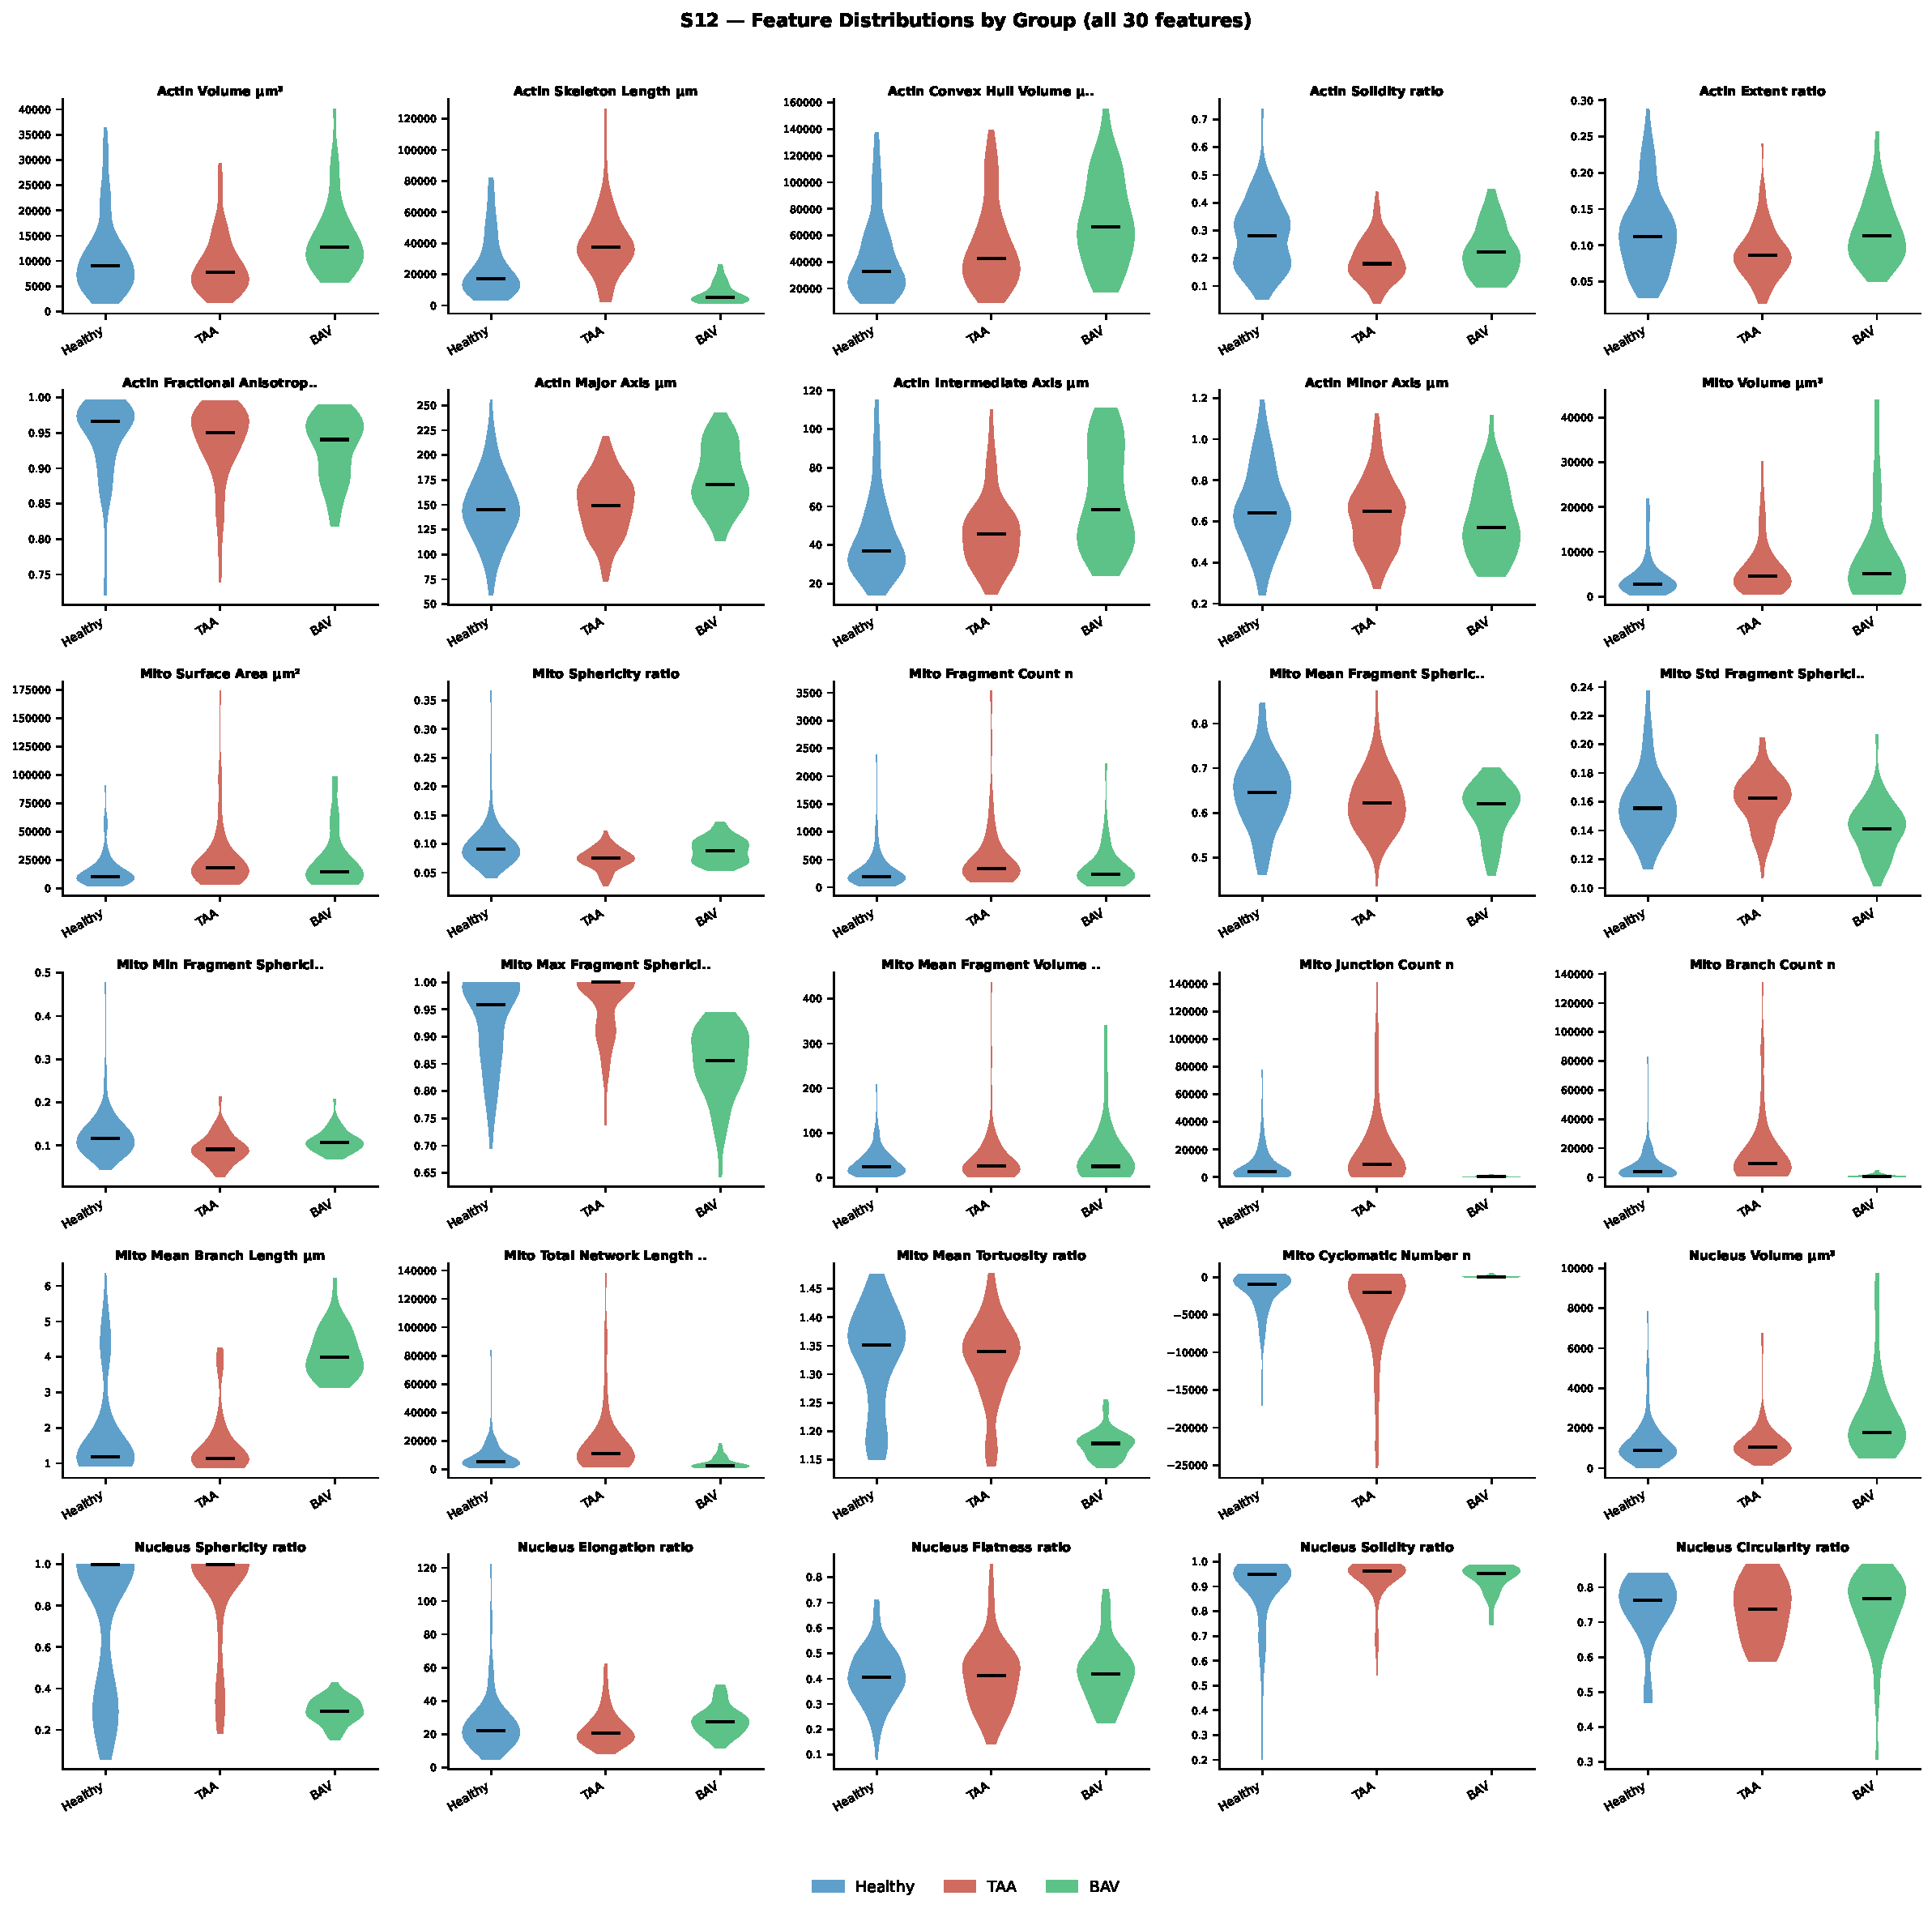
\includegraphics[width=\textwidth]{S12_feature_distributions.pdf}
  \caption*{S12 --- Per-feature distribution by group.}
\end{figure}
\end{document}
